% mnras_template.tex 
%
% LaTeX template for creating an MNRAS paper
%
% v3.0 released 14 May 2015
% (version numbers match those of mnras.cls)
%
% Copyright (C) Royal Astronomical Society 2015
% Authors:
% Keith T. Smith (Royal Astronomical Society)

% Change log
%
% v3.0 May 2015
%    Renamed to match the new package name
%    Version number matches mnras.cls
%    A few minor tweaks to wording
% v1.0 September 2013
%    Beta testing only - never publicly released
%    First version: a simple (ish) template for creating an MNRAS paper

%%%%%%%%%%%%%%%%%%%%%%%%%%%%%%%%%%%%%%%%%%%%%%%%%%
% Basic setup. Most papers should leave these options alone.
\documentclass[fleqn,
% referee, % this line changes to double-spaced 1 column
usenatbib]{mnras}


% MNRAS is set in Times font. If you don't have this installed (most LaTeX
% installations will be fine) or prefer the old Computer Modern fonts, comment
% out the following line
\usepackage{newtxtext,newtxmath}
\usepackage{anyfontsize}
% Depending on your LaTeX fonts installation, you might get better results with one of these:
%\usepackage{mathptmx}
%\usepackage{txfonts}

% Use vector fonts, so it zooms properly in on-screen viewing software
% Don't change these lines unless you know what you are doing
\usepackage[T1]{fontenc}

% Allow "Thomas van Noord" and "Simon de Laguarde" and alike to be sorted by "N" and "L" etc. in the bibliography.
% Write the name in the bibliography as "\VAN{Noord}{Van}{van} Noord, Thomas"


%%%%% AUTHORS - PLACE YOUR OWN PACKAGES HERE %%%%%

% Only include extra packages if you really need them. Common packages are:
\usepackage{graphicx}	% Including figure files
\usepackage{amsmath}	% Advanced maths commands
% \usepackage{amssymb}	% Extra maths symbols
\usepackage{hyperref}
\usepackage[normalem]{ulem}
\usepackage[dvipsnames]{xcolor}
% \usepackage{enumitem}

\usepackage{tikz}


\graphicspath{{figures/}} 
% \linespread{1.8}




%%%%%%%%%%%%%%%%%%%%%%%%%%%%%%%%%%%%%%%%%%%%%%%%%%

%%%%% AUTHORS - PLACE YOUR OWN COMMANDS HERE %%%%%

% Please keep new commands to a minimum, and use \newcommand not \def to avoid
% overwriting existing commands. Example:
%\newcommand{\pcm}{\,cm$^{-2}$}	% per cm-squared


% citations
\defcitealias{james+21}{J21}
\newcommand{\JJ}{\citetalias{james+21}}
\newcommand{\VICE}{\textsc{vice}}


\newcommand{\fruity}{\texttt{\hyperlink{fruity}{Fruity}}}
\newcommand{\nugrid}{\texttt{\hyperlink{nugrid}{NuGrid}}}
\newcommand{\monash}{\texttt{\hyperlink{monash}{Monash}}}
\newcommand{\aton}{\texttt{\hyperlink{aton}{ATON}}}
\newcommand{\cfactor}{1.95}
\newcommand{\nsubgiants}{14,069}

% displays fractions within fractions well
\newcommand{\ddfrac}[2]{\ensuremath{%
    \frac{\displaystyle{#1}}{\displaystyle{#2}}
}}



% Acronyms
\newcommand{\agb}{AGB}
\newcommand{\apogee}{APOGEE}
\newcommand{\aspcap}{\textsc{aspcap}}
\newcommand{\cc}{CCSN}
\newcommand{\gce}{GCE}
\newcommand{\ia}{SN Ia}

% internal abbreviations
\newcommand{\caah}{[C/Mg]-[Mg/H]}
\newcommand{\caafe}{[C/Mg]-[Mg/Fe]}

\newcommand{\Var}{\operatorname{Var}}


% other
\newcommand{\fmeas}{20\%}

\makeatletter
\newcommand{\C}[1][\@nil]{
    \def\tmp{#1}%
    \ifx\tmp\@nnil%
        \ensuremath{\rm C}%
    \else%
        \ifmmode ^{#1}{\rm C}%
        \else $^{#1}$C%
        \fi%
\fi }
\makeatother

\newcommand{\Yct}{{y_{\rm C}}}
\newcommand{\Ycc}{{y_{\rm C}^{\rm CC}}}
\newcommand{\Yoc}{{y_{\rm Mg}^{\rm CC}}}
\newcommand{\Ycagb}{{y_{\rm C}^{\rm AGB}}}
\newcommand{\ycagb}{\y_{\rm C}^{\rm AGB}}
\newcommand{\aagb}{\alpha_{\rm C}^{\rm AGB}}
\newcommand{\zagb}{\zeta_{\rm C}^{\rm AGB}}
\newcommand{\zcc}{\zeta_{\rm C}^{\rm CC}}
\newcommand{\noneqagb}{\nu_{\rm C}^{\rm AGB}}
 \newcommand{\yb}{\ensuremath{\rotatebox[origin=B,y=0.5ex]{180}{y}}}
\newcommand{\y}{p}
\newcommand{\fagb}{f_{\rm C}^{\rm AGB}}

\newcommand{\zetao}{\zeta_0}
\newcommand{\zetai}{\zeta_{1}}
\newcommand{\zetaii}{\zeta_{2}}
\newcommand{\Zl}{x_{\rm low}}

\newcommand{\Mo}{ {\rm M}_{\sun}}
    
\newcommand{\Zo}{ Z_{\sun}}

\newcommand{\about}[1]{${\sim} #1$}

%%% citepos command
\makeatletter
\DeclareRobustCommand\citepos
  {\begingroup
   \let\NAT@nmfmt\NAT@posfmt% ...except with a different name format
   \NAT@swafalse\let\NAT@ctype\z@\NAT@partrue
   \@ifstar{\NAT@fulltrue\NAT@citetp}{\NAT@fullfalse\NAT@citetp}}

\let\NAT@orig@nmfmt\NAT@nmfmt
\def\NAT@posfmt#1{\NAT@orig@nmfmt{#1's}}

\makeatother


% Caption macros
\newcommand{\captionline}[2][very
thick]{\tikz[baseline={([yshift=-.5ex]current bounding box.base)}]{
\draw[#2,#1, line cap=round] (0,0) -- (0.3,0); }}




%%%%%%%%%%% JWJ' editing macros %%%%%%%%%%%
\newcommand{\strike}[1]{{\color{ForestGreen} \sout{#1}}}
\newcommand{\add}[1]{{\color{ForestGreen} #1}}
\newcommand{\note}[1]{{\color{ForestGreen} \textit{ \small (JWJ: #1)}}}
% \LetLtxMacro\origcitep\citep
% \LetLtxMacro\origcitet\citet
% \renewcommand{\citep}[2][]{%
%     \mbox{\origcitep[#1][]{#2}}
% }
% \renewcommand{\citet}[2][]{%
%     \mbox{\origcitet[#1][]{#2}}
% }

\newcommand{\dbstrike}[1]{{\color{Thistle} \sout{#1} }}
\newcommand{\dbadd}[1]{{\color{Thistle} #1}}
\newcommand{\dbnote}[1]{ {\color{Thistle} \textit{\small (DB: #1)}} }


% \LetLtxMacro\origcite\cite

% This is my command. I want to strike out, 
% \newcommand{\strikeit}[1]{%
%   \ifcorrectingmode
%   \mbox{\sout{#1}}%
% %  \makebox[\textwidth][s]{\sout{#1}}%
%   \fi
% }

% \renewcommand{\cite}[2][]{%
%   \ifcorrectingmode
%   \mbox{\origcite[#1]{#2}}%
%   \else
%   \origcite[#1]{#2}%
%   \fi
% }




%%%%%%%%%%%%%%%%%%%%%%%%%%%%%%%%%%%%%%%%%%%%%%%%%%

%%%%%%%%%%%%%%%%%%% TITLE PAGE %%%%%%%%%%%%%%%%%%%

% Title of the paper, and the short title which is used in the headers.
% Keep the title short and informative.
\title[The Origin and Galactic Evolution of Carbon]{The Galactic Chemical Evolution of Carbon: Implications for Stellar Nucleosynthesis }

% The list of authors, and the short list which is used in the headers.
% If you need two or more lines of authors, add an extra line using \newauthor
\author[D. A. Boyea et. al.]{%
Daniel A. Boyea,$^{1, 2, 3}$\thanks{%
Contact e-mail:~\href{mailto:boyea.2@osu.edu}{boyea.2@osu.edu}}
James W. Johnson,$^{1, 2, 4}$
Third Author$^{2,3}$
and Others$^{1,3}$
\\
% List of institutions
$^{1}$Department of Astronomy, The Ohio State University, 140 W. 18th Ave., Columbus, OH, 43210, USA
\\
$^{2}$Center for Cosmology \& Astroparticle Physics (CCAPP), The Ohio State University, 191 W. Woodruff Ave., Columbus, OH, 43210, USA
\\
$^{3}$Department of Physics \& Astronomy, University of Victoria, Victoria, BC V8P 5C2, Canada
\\
$^{4}$The Observatories of the Carnegie Institution for Science, 813 Santa Barbara St., Pasadena, CA, 91101, USA
}

% These dates will be filled out by the publisher
\date{Accepted XXX. Received YYY; in original form ZZZ}

% Enter the current year, for the copyright statements etc.
\pubyear{2025}

% Don't change these lines
\begin{document}
\label{firstpage}
\pagerange{\pageref{firstpage}--\pageref{lastpage}}
\maketitle



% Abstract of the paper
\begin{abstract}
% context
The astrophysical origin of carbon remains largely uncertain---different studies propose that either asymptotic giant branch (AGB) stars or core collapse supernovae (CCSNe) may be the dominant process.
% 
We aim to constrain the stellar yields of C through multi-zone Galactic chemical evolution models by comparing predictions with \apogee\ subgiants abundances.
% 
We show \caah\ trend represents the equilibrium abundances of C and Mg, deriving the total C yield as a function of metallicity. 
Instead, the \caafe\ trend (at a given metallicity) is an empirical estimate of the delay time distribution of C.
We infer that AGB stars produce between 10 and 40\% of C. Additionally, we show that all AGB models produce C too quickly, and the low-mass AGB C yield is likely underestimated. 
% misc
Our models are relatively independent of uniform scaling of yields and outflows, and alternate star formation histories. 
However, the stars which contribute to \agb\ C production and the \ia\ delay time distribution of Fe contribute uncertainties to our conclusions. 
% gas phase
While reliable gas-phase and low-metallicity measurements of C are challenging, we find that our model and a single-zone model with our recommended yields replicate the broad trends of \caah{} across different environments and metallicities. 

\end{abstract}

\begin{keywords}
galaxies: abundances -- galaxies: evolution -- galaxies: star formation -- galaxies: stellar content -- methods: numerical
\end{keywords}



%%%%%%%%%%%%%%%%%%%%%%%%%%%%%%%%%%%%%%%%%%%%%%%%%%

%%%%%%%%%%%%%%%%% BODY OF PAPER %%%%%%%%%%%%%%%%%%

\section{Introduction}


\begin{figure*}
    \centering
    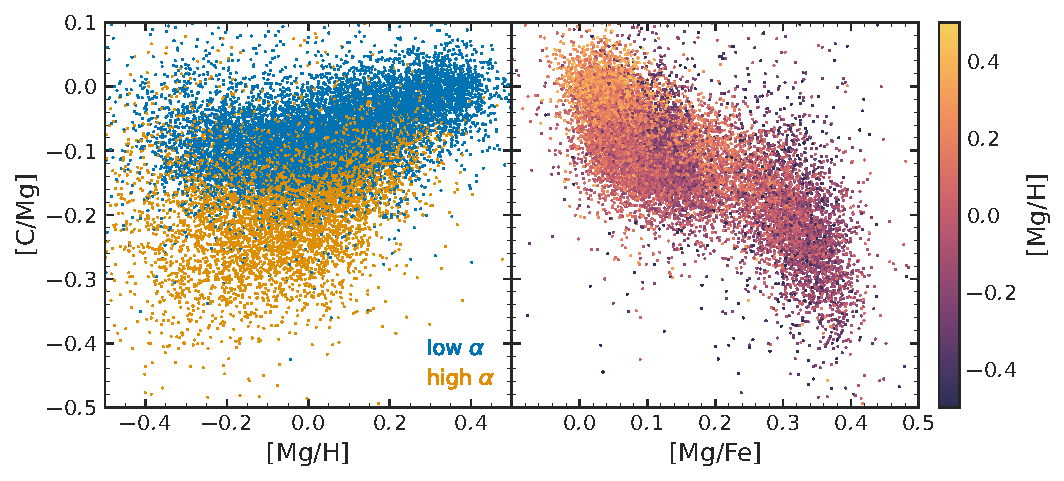
\includegraphics{subgiants.pdf}
    \caption{The [C/Mg] ratio against [Mg/H] (left) and [Mg/Fe] (right) for the \citet{jack}~sample of \apogee{} subgiants. On the left, we plot high and low-$\alpha$ stars in blue and orange, using the separation defined in Eq.~\ref{eq:high_alpha}.  On the right, we colour-code stars according to their [Mg/H] abundance. The median subgiant trends serve as our emperical benchmark. } \label{fig:subgiants}
\end{figure*}



Despite being the most abundant metal in the Universe~\citep[e.g.][]{magg+22}, the nucleosynthetic origin of C is poorly understood. 
There is broad agreement that both high mass and asymptotic giant branch (AGB) stars produce C \citep{jennifer19}, but their relative yields are disputed.
From a Galactic chemical evolution (GCE) perspective, some authors have argued that high-mass stars should dominate~\citep[e.g.][]{prantzos+94, HEK00, romano+20, franchini+20, gustafsson22}, and others have argued that AGB stars should contribute at least half of the C in the universe~\citep[e.g.][]{tinsley79, chiappini+03, mattsson10, KKU11, rybizki+17, KKL20}. 
In this paper, we aim to constrain C production using subgiant stars and multi-zone GCE models.% \dbstrike{incorporating stellar radial migration}.

% Formed in the cores of stars during He fusion, C is the first \dbadd{primary? element} after He. Additionally, C is one of the only light elements formed in low-mass stars \citep[e.g.,][]{KL14}. \dbnote{I don't like how many e.g.'s there are, and is this the right citation here?}
%\dbadd{
% Because the effects of first dredge up are mass-dependent, C and N abundances are frequently used as age indicators for RGB stars \citep{MG15, martig16, hasselquist19, vincenzo+21}. 
% }
% \dbnote{C abundnces for stellar structure (opacities) and star formation (line cooling)}
% \dbadd{In addition, stellar parameters such as convection and mass loss are calibrated to match observed stars and cannot be predicted from first principles.} \dbnote{need to check if this means SE models are calibrated to match yields or just stellar parameters.}


Predictions of C yields from stellar evolution and supernova (SN) models are riddled with uncertainties (see, e.g., the reviews by \citealt{romano+10, KL14}).
Some salient unknowns include mass loss rates \citep{sukhbold+16, beasor+2020}, rotational mixing \citep{frischknecht+16, LC18}, nuclear reaction rates \citep{herwig+05, herwig+austin2004}, and convection \citep{chieffi2001, ventura+13}.
Recent work additionally suggests that small changes in a stars's initial mass of 
 $\sim$$0.01 M_\odot$  have significant effects on the evolution and explosion outcomes of massive stars \citep{bruenn+2023, vartanyan_burrows2023}.
 Furthermore, many stars are found in binary systems \citep{sana+12}, the effects of which are almost entirely
unexplored in stellar nucleosynthesis models \citet{farmer+21}.
Accurate predictions of metal yields from stellar evolution models remain elusive.

Given the challenge of theoretical yield predictions, recent work aims to empirically characterize elemental production. \dbnote{are there older relevant references like garnett1997? or other relevant work (eitner+20?)}
\citet{weinberg+19, weinberg+22} analyzed the abundance ratio trends of high- and low-alpha sequence stars in APOGEE~\citep{apogee17} to infer relative yields of prompt and delayed enrichment sources and their metallicity dependence.
\citet{emily+19, emily+22, emily+24} applied the same methodology to GALAH~\citep{DeSilva2015, Martell2017}.
\citet{rodriguez+21, rodriguez+23} measured the mean Fe yield of core-collapse supernovae (CCSNe) using the radioactive tails of their lightcurves.
Their measurements, provide one of few empirical anchors on the absolute scale of yields \citep{david_fe}.


 % Folowing many previous works  (e.g. \citealt{DTS78, BF06, prantzos+18, berg+19}; see also the recent reviews by \citealt{romano22} and \citealt{RM21}.) this paper focuses on the evolution of C in GCE models.
\citet{james+24} recently argued that the enrichment history of the Galactic disk can be described as an equilibrium phenomenon.
In equilibrium GCE, trends in abundance ratios closely trace yield ratios (see their section 5.2.2).
\citet{james+23} had previously shown that the correlation between gas-phase N and O abundances (see their Fig. 1) could be described as a consequence of the metallicity dependence of the relative N and O yields.
Under their equilibrium scenario, this argument should extend to any element whose enrichment by stellar populations does not require long timescales ($\gtrsim$few Gyr).
We show in section~\ref{sec:agb} that the characteristic delay times of C production should be $\sim$ 1 Gyr, within this limit. 
\dbnote{This is complicated by the difference between high alpha and low alpha, and 1-2Msun stars do produce carbon.... Also, I would like to call out reviews and general works on C at some point.}


We use a sample of subgiant stars from APOGEE \citep{apogee17} as our primary observational constraint.
APOGEE Subgiants provide a large, homogeneous sample of well-measured C abundances unaffected by stellar evolution.
\dbadd{Subgiants' photospheric C abundance closely matches their birth composition.}
\dbstrike{Subgiants have the advantage that their photospheric abundances of C directly reflect their birth C abundances much more closely than other spectral types.} \citep{gilroy89, korn+07, lind+08, souto+18, souto19}.
In other evolutionary phases, the measured abundances are known to be affected by internal processes (see discussion in section~\ref{sec:data_selection} below).
Our sample should therefore be unaffected by uncertainties with inferring their birth abundances.



In section~\ref{sec:data_selection} we describe the selection for our subgiant observational sample.
In section~\ref{sec:nucleosynthesis}, we discusses theoretical estimates of \agb\ and \cc\ C yields and present the yield prescriptions we use for our models.
In section~\ref{sec:vice}, we describe the remaining details of our GCE models.
In section~\ref{sec:results}, we present our model predictions and discuss their observationally distinguishable predictions. 
In section~\ref{sec:gas}, we compare our model to observations of halo stars and extragalactic HII regions from the literature. 
We summarize our conclusins in section~\ref{sec:conclusions}.





% \footnotetext{\strike{By metallicity, we mean the (mass) fraction of any element which is not H or He, denoted by $Z$. For the sun, we take $Z_\odot=0.0176$.} }


\section{The Subgiant Sample}\label{sec:data_selection}




% Subgiants are a useful empirical benchmark because their photospheric abundances should reflect their birth mixture. 
We use subgiant stars as our empirical benchmark.
Subgiants have the advantage that their photospheric C and N abundances should closely approximate their birth mixture.
During main sequence evolution, metals can fall below the convective envelope (\textit{gravitational settling}; e.g. \citealt{turncotte+98}).
When stars evolve off main sequence and become subgiants, these metals are reincorporated into the convective envelope \citep[]{gratton+00, souto19}. 
However, once a star becomes a red giant, \textit{first dredge up} pollutes its photosphere with core, CNO-processed material
\citep{iben67, KL14}. 
\dbnote{Is there other justification for subgiants? Consistent stellar parameters, subgiant spectra are easier than white dwarfs? only a $\sim 0.05$ dex correction}

We use the sample of \apogee\ DR17 subgiants from \citet{jack}. We select stars from the ASPCAP pipeline (revision 1) within the $\log g$-$T_\text{eff}$ polygon given by
 \begin{equation}
    \begin{cases} \label{eq:subgiant_selection}
        \log \text{g} \geq 3.5 \\
        \log \text{g} \leq 0.004\,T_{\rm eff} - 15.7 \\
        \log \text{g} \leq 0.0007\,T_{\rm eff} + 0.36 \\
        \log \text{g} \leq -0.0015\,T_{\rm eff} + 12.05 \\
        \log \text{g} \geq 0.0012\,T_{\rm eff} - 2.8. \\
    \end{cases}
\end{equation}
Following \citet{jack}, we also exclude stars with the flags:
        \verb|APOGEE_MIRCLUSTER_STAR|,
        \verb|APOGEE_EMISSION_STAR|,
        \verb|APOGEE_EMBEDDEDCLUSTER_STAR|,
        \verb|APOGEE2_YOUNG_CLUSTER|,
        \verb|APOGEE2_W345|,
        \verb|APOGEE2_EB|, and
        \verb|DUPLICATE|.
We additionally remove stars with no reported (or flagged unreliable), C, Mg, or Fe abundances. These cuts yield a sample containing \nsubgiants\ subgiants.


Fig.~\ref{fig:subgiants} shows out subgiant sample plotted in the \caah\ and \caafe{} planes.\footnotemark{} In this sample, [C/Mg] increases with [Mg/H], and [C/Mg] decreases with [Mg/Fe] at fixed [Mg/H]. Our aim is to reproduce these trends.


\footnotetext{In this paper, we use the standard notation for chemical abundances. $[A/B] = \log_{10}\left(A/B\right) - \log_{10}\left(A_{\sun}/B_{\sun}\right)$, i.e. $[A/B]$ is the logarithm of the mass ratio between A and B, scaled such that $[A/B]=0$ for the sun (see Table~\ref{tab:fiducial_mod} for solar scale.) }

We have also investigated these thrends in other catlogues (not show) in order to understand the systematic uncertainties of our APOGEE subgiant sample.
Namely, we we consider subgiants/dwarfs from GALAH DR4 \citep{galah_dr4}, Gaia-ESO DR5.1 \citep{gaiaeso_dr5.1}, and LAMOST \citep{lamost} with similar selection criteria. Additionally, we consider APOGEE Giants with first dredge up mixing corrections from \citep{vincenzo+21}.
In general, different surveys follow similar trends in \caah\ and \caafe\ but with systematic offsets at the $\sim{0.1}$ dex level in [C/Mg] given [Mg/H] and slight variations in the slope.
These systematic differences are not a major concern for our conclusions since our models are mostly constrained by the slope of \caah\ and \caafe,  not their normalization (see Fig.~\ref{fig:zeta_f} and discussion in section \dbadd{5.2}).

\section{Nucleosynthesis}\label{sec:nucleosynthesis}

A yield quantifies the new production of a chemical species. For a given star, we define the {\it stellar yield of $X$} as the fraction of a star's initial mass synthesized into a new element, $X$. Specifically, the stellar yield of $X$ is
\begin{equation} \label{eq:stellar_yield_def}
   \y_{\rm X}(m, Z) := 
    \frac{m_{X, \rm ej}- Z_{X,\rm  ini}\,m_{\rm ej}}{m}
\end{equation}
where $Z_{X,\rm ini}$ is the initial mass abundance of $X$, $m_{\rm ej}$ is the ejected mass, $m_{X, \rm ej}$ is the ejected mass of $X$, and $m$ is the initial mass of the star.
Note that yields may become negative if more X is transformed into other elements than is produced.
We also describe yields by their population-averaged quantities, {\it integrated yields}, the amount of newly produced X per unit mass of star formation. 
The integrated yield of $X$ is
\begin{equation} 
   y_{X}(Z) := 
    \frac{M_X - r\,Z_{X, \rm ini}\,M_{\rm ssp}}{M_{\rm ssp}},
\end{equation}
where $M_X$ is the total expelled mass of element X, $M_{\rm ssp}$ is the birth mass of the single stellar population (SSP)\footnote{An SSP is a cluster of stars born at the same time from the same material.}, and $r$ is the return fraction (fraction of the SSP mass returned to the interstellar medium). 

Table~\ref{tab:fiducial_mod} summarizes our yield choices. 
Following \citet{james+23}, we integrate yields and our GCE models using the publicly available Versatile Integrator for Chemical Evolution (\VICE, \citealt{JW20}). We use the O, Mg, and Fe yields recommended by \citet{david_fe} based on measurements of the mean CCSN Fe yield \citep{rodriguez+23} and APOGEE chemical abundances.
Our N yield is scaled from \citep{james+23}.
We assume a \citet{kroupa01} initial mass function (IMF).


\begin{table}
	\centering
    \caption[]{Solar abundance scale and fiducial yields (in units of stellar population birth mass). See section \ref{sec:agb} for the definition of \fruity. The solar abundance scale is \citet{magg+22} + 0.04 dex suggested by \citet{david_fe}.
    \dbnote{any tips to make this table a little bit smaller?}
    }
	\label{tab:fiducial_mod}

	\begin{tabular}{l l l l l}
		\hline
         & $Z_{X,\,\sun}$ & $y_X^{\rm cc}$ & $\y_X^{\rm agb}$ & $y_X^{\rm ia}$  \\
		\hline
        C & $33.9\times10^{-4}$ & Eq.~\ref{eq:y_cc} & $\cfactor\times$\fruity &  0 \\
        O & $73.3\times10^{-4}$ & $71.3\times10^{-4}$ & 0 & 0 \\
        Mg & $6.71\times10^{-4}$ & $6.52\times 10^{-4}$ & 0 & 0 \\
        Fe & $13.7\times10^{-4}$ & $4.73\times10^{-4}$ & 0 & $7.82\times10^{-4}$ \\
        N & $10.4\times10^{-4}$ & $5\times10^{-4}$ & $5\times10^{-4}M\left(\frac{Z}{Z_\odot}\right)$ & 0\\
		\hline
	\end{tabular}
\end{table}


\subsection{Asymptotic Giant Branch Stars}\label{sec:agb}

\begin{figure*}
    \centering
 	    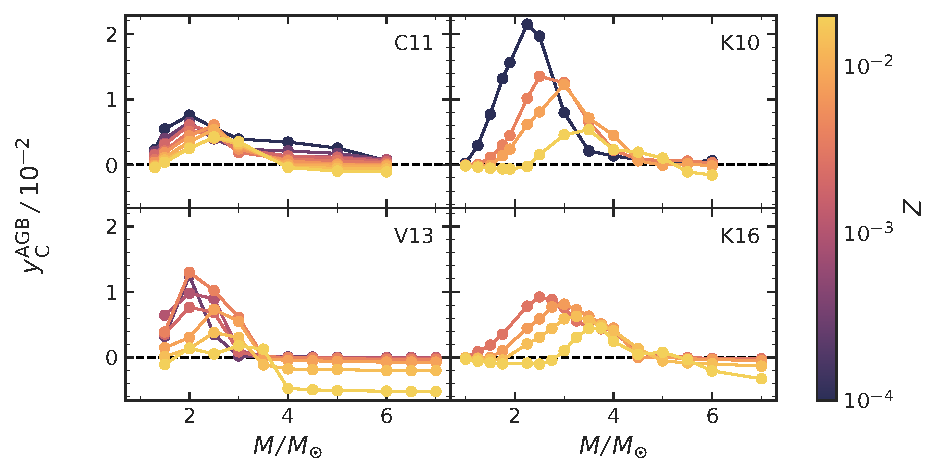
\includegraphics[scale=1]{agb_yields.pdf}
        \caption[]{The net fractional \agb\ C yield  plotted as a function of initial stellar mass and colour-coded according to metallicity. The black dashed line shows $\Ycagb=0$ for reference. Each panel represents yields from one of four \agb\ models: \fruity{}, \aton{}, \monash{}, \nugrid{} (see sections \ref{sec:agb}) }.

        \label{fig:y_agb}
\end{figure*}

\begin{figure*}
    \centering
    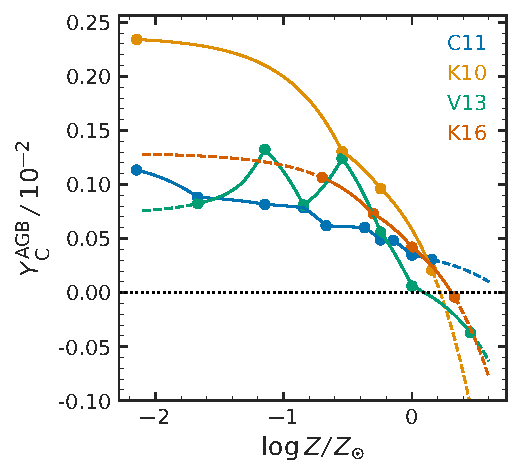
\includegraphics{y_agb_vs_z.pdf}
    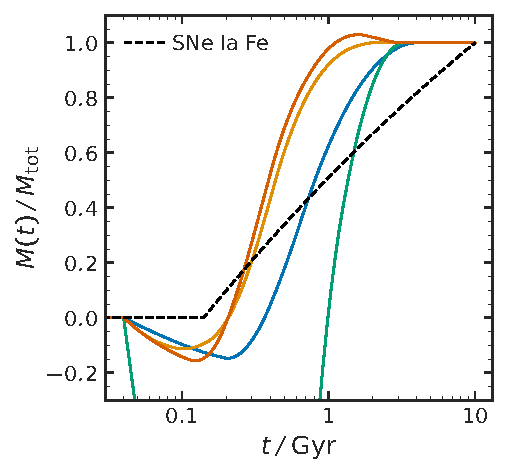
\includegraphics{y_agb_vs_t.pdf}

    \caption[]{\textbf{Left} The integrated \agb\ C yield $\Ycagb$ as a function of metallicity for each of the \agb\ yield tables.
    \textbf{Right} cumulative C return fraction as a function of age for a solar metallicity single stellar population. The dashed black line shows the cumulative return fraction of type Ia supernovae ($\propto t^{-1.1}$) for comparison. The minimum of \aton{} is at $y( 0.30\,{\rm Gyr})/y(t_{\rm end})=-7.81$ and is large as the net yield is close to zero.
}

    \label{fig:agb-ssp}

\end{figure*}


An asymptotic giant branch (AGB) star is a low mass star undergoing He shell burning, the last nuclear phase (see e.g. \citealt{PR2023}). AGB stars enrich the interstellar medium (ISM) through mass expelled during thermal pulses. 


We explore four different stellar AGB yield tables from the literature which provide well-sampled grids in mass and metallicity. We refer to the tables as 
\begin{description}
    \item \hypertarget{fruity}{\texttt{FRUITY}}: \citet{cristallo+11, cristallo+15}
    \item \hypertarget{aton}{\texttt{ATON}}: \citet{ventura+13,ventura+14,ventura+18, ventura+20}
    \item \hypertarget{monash}{\texttt{Monash}}: \citet{KL16, karakas+18}
    \item \hypertarget{nugrid}{\texttt{NuGrid}}: \citet{pignatari+16, ritter+18, battino+19, battino+21}
\end{description}
Each AGB yield table reports yields for stellar models on a grid of masses and metallicities as reported in Table~\ref{tab:agb}.
We use the same tables as \citet{james+23}, except that we have swapped \citet{karakas10} for \citet{pignatari+16}. (See section~\ref{sec:nugrid_yields} for the implementation and recalculation of these yields.)
For our models to better match observations, we uniformly amplify the yield tables according to
\begin{equation} \label{eq:alpha}
        \ycagb(m, Z) \rightarrow \alpha_{\rm agb}\ \ycagb(m, Z).
\end{equation}
We use the \fruity\ table, with $\alpha_{\rm agb}=\cfactor$, as the fiducial \agb\ yield.

Fig.~\ref{fig:y_agb} compares the C yields for these four AGB models.
Most models agree on general yield trends in mass and metallicity.
C production peak between masses of $\sim$ 2--4 $\Mo$. As metallicity increases, the net yield decreases and the mass of peak C production increases slightly.


In order to integrate AGB yields with \VICE, we linearly interpolate yield tables in both mass and metallicity. Below the smallest mass in a table, $\ycagb$ is linearly extrapolated to 0 at $1\Mo$. The population-averaged AGB star yield is calculated with 
\begin{equation} \label{eq:imf-agb-yield}
    y_{X}^{\rm AGB}(Z,\tau) = 
    \int^{u_{\rm AGB}}_{m_\textrm{post-AGB}(\tau)} 
    \y_{\rm X}(m, Z)\ 
    \frac{1}{A}\frac{dN}{dm}\ m\ dm
\end{equation}
are the minimum and maximum mass of star formation, $u_{\rm AGB}=8\Mo$ is the maximum mass of an AGB star, $m_\textrm{post-AGB}(\tau)$ is the mass of stars which complete AGB evolution at age $\tau$, and $dN/dm$ is the initial mass function (IMF). The IMF normalization is
\begin{equation} \label{eq:imf_normalization}
    A := \int_l^u m \frac{dN}{dm} dm
\end{equation}
    where  $l=0.08\,\Mo$ and $u = 100\,\Mo$ are the assummed minimum and maximum mass of star formation. We assume a \citet{larson74} mass-lifetime-relationship and assume that the total lifetime (through post-AGB) is $1.1\times$ the main sequence lifetime.


The left panel of Fig.~\ref{fig:agb-ssp} shows IMF-averaged C yields for each \agb\ model as a function of metallicity.
The IMF-averaged yields differ in normalization and metallicity dependence.  
The normalizations span a factor of \about{2}. (e.g. between $6\times 10^{-4}$ and $12 \times 10^{-4}$ at $Z=0.33\,\Zo$)
Both \nugrid{} and \aton{} predict non-monotonic C yields with $Z$, but AGB modeling uncertanties may eclipse this prediction's significance. To characterize the metallicity dependence of each table, we fit the yield to a linear model in $\log Z$
\begin{equation}\label{eq:agb_z_approx}
    y_{\rm C}^{\rm AGB}(Z) = \zetao^{\rm AGB} + \zetai^{\rm AGB} \log(Z / \Zo).
\end{equation}
Table \ref{tab:agb} also contains the linear fit parameters for each AGB table.
The values of $\zagb$ span a factor of $\sim{3}$ between models.
These variations are due to different choices of reaction rates, convection treatments, and mass-loss rates (see discussion below and \JJ). 



The right panel of Fig.~\ref{fig:agb-ssp} shows the total relative production of C by \agb\ stars by a solar metallicity SSP as a function of age.
As the mass range $2\,\Mo\lesssim M \lesssim 4\,\Mo$ is predicted to be most important for C production, half the yield is produced before \about{1}\,Gyr, similar to Fe production by \ia. 
\monash{} weights C production more heavily towards high-mass \agb\ stars, resulting in shorter delay times, whereas the \fruity\ model predict a slightly longer timescale of \about{1}\,Gyr. In any case, little to no C is produced more than 2\,Gyr after a star formation event. Fe production, in contrast, continues steadily for 10\,Gyr. 

In AGB stars, {third dredge up} (TDU) and {hot bottom burning} (HBB) are two competing processes driving C evolution.
TDU accompanies thermal pulses, where material from the CO core is mixed with the envelope, increasing surface C abundances 
later released to the ISM \citep{KL14}.  
HBB\ is the activation of the CNO cycle at the bottom of the convective envelope.
TDU increases C yields and HBB converts C into N. 
%Because the $^{14}$N proton capture is the slowest component of the CNO cycle, the CNO cycle converts nearly all \C[12] into $^{14}$N \citep{solar-fusion}.

% \footnotetext{
%     The CNO cycle is a series of proton-capture reactions with CNO elements resulting in energy generation and the creation of an $\alpha$ particle. $\C[12]({\rm p}, \gamma)
%     ^{13}{\rm N}(\beta^+, \nu_{\rm e})
%     ^{13}{\rm C}({\rm p}, \gamma)\allowbreak
%     ^{14}{\rm N}({\rm p}, \gamma)\allowbreak
%     ^{15}{\rm O}(\beta^+, \nu_{\rm e})\allowbreak
%     ^{15}{\rm N}({\rm p}, \alpha)
%     \C[12]$. 
% There are other less important minor branches of the CNO cycle
%  \citep{solar-fusion}.
% }


Both HBB and TDU result in mass and metallicity dependent C yields. 
Stars less than \about{2}\,$\Mo$ do not experience TDU. As a result, C yields from these stars are affected only by first dredge-up, resulting in small net C yields \citep[Table 1]{karakas10}.
Above \about{2}\,$\Mo$, TDU becomes important, enriching the outer layers with C.
In \agb\ stars more massive than \about{5}\,$\Mo$, efficient HBB turns most \C[12] into $^{14}$N.
TDU is more efficient for compact, massive cores. HBB requires a more massive AGB star to reach sufficient temperatures at the base of the convective envelope to initiate CNO. Both processes are more efficient at low metallicity due to the lower opacities, hotter temperatures, and more compact internal structures. The details of each process are ultimately set by the uncertain choices for stellar evolution models.

% compactness causes stronger thin-shell instability
% C yields increase because TDU outweights HBB when low Z.


The primary uncertainties in AGB stellar evolution are convection, nuclear reaction rates, and mass loss prescriptions.
\citet{ventura+15} compared the \aton{} and \monash{} models, finding that differences in yields are primarily driven by differences in mass-loss and convection prescriptions. \aton{} predicts strong HBB to set in $\sim{1}\,\Mo$ lower than in \monash{}, leading to much lower C yields.
Moreover, the $^{14}{\rm N}({\rm p},\gamma)$ reaction rate uncertainty causes a factor of 2 difference in predicted C yields \citep{herwig+austin2004, HAL2006}.
Most of the physics included in stellar modelling is empirically calibrated. Mass-loss rates, convection, and extra mixing are not sufficiently well understood to be computed from first principles.

Super AGB stars are the class of AGB stars with masses $\sim8$ to $\sim10\Mo$ which burn O into Si and Mg. While we neglect super-AGB stars in the discussion above, these stars are not predicted to be substantial producers of C, similar to high mass AGB stars. From the \citet{doherty+14, doherty+14b} yield table (extending the \monash\ yields), the highest net fractional yield is only -0.002 for super solar metallicity, which would have a negligible impact on the integrated yield). Additionally, as discussed in section~\ref{sec:degeneracies} below, the short lifetimes of high mass AGB and super-AGB stars mean they have minimally affect our conclusions and can be grouped with CCSNe yields.


\begin{table*}
	\centering
    \caption[]{For each \agb\ yield set, the IMF-averaged \agb\ C yield at solar metallicity $y_{\rm C, 0}^{\rm AGB}$, the linear fit solar yield $\zetao$ and slope $\zetai$ (see Eq.~\ref{eq:agb_z_approx}), the fraction of solar C produced in the model $f_\odot^{\rm AGB}$, and the masses and metallicities each yield table is sampled on.
    $f_{\rm odot}^{\rm AGB}$ is calculated based on $\zetao$ assuming a total C yield of $\Yct = 0.00275$.
    }

	\label{tab:agb}
    \begin{tabular}{c  ccc  c p{4cm} p{4cm}} % four columns, alignment for each
		\hline 
        \agb\ table 
                & $y_{\rm C, \odot}^{\rm AGB}\times10^4$ %& y
                & $\zetao^{\rm AGB}\times 10^4$ %& y
                & $\zetai^{\rm AGB}\times 10^4$
                &  $f_\odot^{\rm AGB}$
                & masses ($\Mo$) & metallicities ($Z$)\\
        \hline
        \fruity 
                & 3.229
                &  $3.8\pm0.3$
                & $-3.5\pm0.3$
                & 0.14
                & 1.3, 1.5, 2, 2.5, 3, 4, 5, 6
                & 0.0001, 0.0003, 0.001, 0.002, 0.003, 0.006, 0.008, 0.01, 0.014, 0.02
                \\
        \aton 
                & 0.2851
                & $1.4\pm1.8$
                & $-10. \pm 3$
                & 0.05
                & 1.5, 2, 2.5, 3, 3.5, 4, 4.5, 5, 6, 6.5, 7
                & 0.0003, 0.001, 0.002, 0.004, 0.008, 0.014, 0.04
                \\
        \monash 
                &  3.444
                & $2.8 \pm 0.5$
                & $-11.0\pm 1.0$
                & 0.10
                & 1, 1.25, 1.5, 1.75, 2.25, 2.5, 2.75, 3, 3.25, 3.5, 3.75, 4, 4.5, 5, 5.5, 6, 7 
                & 0.0028, 0.007, 0.014, 0.03
                \\
        \nugrid 
                & 10.95
                & $8.3\pm 1.9$
                & $-4.6\pm1.7$
                & 0.30
                & 1, 1.65, 2, 3, 4, 5, 6, 7
                &  0.0001, 0.001, 0.006, 0.01, 0.02
                \\
		\hline
	\end{tabular}
\end{table*}




\subsection{Core Collapse Supernovae}


Massive stars form $^{12}$C in their cores through the triple-$\alpha$ reaction (He-burning) which is later released to the ISM through winds and supernovae.

We approximate massive star enrichment as occurring instantaneously after a star formation event. Under this approximation, the yield is simply a constant  of proportionality between the metal production rate and the SFR:
\begin{equation}
    \dot{M}_X^{\rm CC} = y_{X}^{\rm CC}\, \dot{M}_\star
\end{equation}
The CCSN integrated yield is given by
\begin{equation}
y_{X}^{\rm CC} = \int_{l_{\rm CC}}^{u} \left[E(m) m_{X\rm, SN} + w_X - Z_X\,(m-m_{\rm rem})\right]\,\frac{1}{A} \frac{dN}{dm}\ dm
\end{equation}
where $E(m)$ is the fraction of stars of mass $m$ which explode, $m_{X,\rm SN}$ and $w_X$ are the mass of $X$ ejected in a CCSN explosion and through stellar winds respectively, $Z_X$ is the initial abundance of $X$, $dN/dm$ is the IMF, $l_{\rm CC}=8\Mo$ is the initial minimum mass of a CCSN progenitor. 
%\dbstrike{We integrate yields using \VICE's {\tt vice.yields.ccsne.fractional} function.} \dbnote{is this too detailed?}

Fig.~\ref{fig:y_cc} shows the integrated yields of several massive star yield models from the literature. 
\cc{} models predict a wide range of C yields, spanning nearly a factor of ten. 
 The \cite{LC18} models, which include rotation, show that the induced mixing (e.g. \citealt{frischknecht+16}) can dramatically increase the magnitude and metallicity dependence of $\Ycc$. As we will later emperically show, \cc\ C production needs to be strongly metallicity-dependent at $Z \approx \Zo$, which is consistent with \citepos{LC18} rapidly rotating models and to a lesser extent \citet{NKT13}.
The left panel of Fig.~\ref{fig:y_cc} also shows the IMF-averaged \agb\ star yields from the \fruity\ model (in Fig.~\ref{fig:agb-ssp}). Especially at $Z\approx Z_\odot$, most \cc\ models dominate \agb\ C production. 


The right panel of Fig.~\ref{fig:y_cc} shows the average [C/Mg] ratio of \cc\ ejecta for the different models, given by
\begin{equation}\label{eq:c_mg_cc}
    {\rm [C/Mg]^{CC}} = \log_{10}\left( \frac{\Ycc}{\Yoc}\right) - \log_{10} \left( \frac{Z_{{\rm C},\ \sun }}{Z_{{\rm Mg},\ \sun }} \right).
\end{equation}
The models we have considered here predict [C/Mg]$^{\rm CC}$ ratios that closely trace the metallicity-dependence of the C yield, a consequence of approximately
metallicity-independent Mg production \citep[e.g][]{andrews+17}.




As opacity increases with metallicity, high-mass stars experience stronger winds. In particular, C enriched envelop material is lost through winds before conversion into heavier elements, resulting in $Z$-dependent C production \citep{LC18}.
While there are many stellar models providing predictions of \cc{} yields, the results of these models are highly uncertain. Furthermore, rotation, binarity, and explodability introduce substantial uncertainties in \cc\ predictions \citep{farmer+21}.

The oxygen-magnesium problem is a know problem where Mg tends to be under-produced in CCSN models relative to 
 O (see discussion in \citealt{emily+21}). Because we update our solar mixture to \citet{magg+22}, the O and Mg abundances of the sun are closer to predictions of CCSN models compared to \citet{asplund+09} solar scale. 
To avoid this problem in our \gce\ models, we simply assume the O and Mg yields from massive stars reflect the solar mixture, consistent with observations from \apogee\ \citep{weinberg+19, weinberg+22, david_fe}. We are more focused on relative yields and trends than the scale of yields. Surveys also have \about{0.1} dex systematic offfsets for a variety of reasons in [C/Mg]. 

To simplify the exploration of C yields from \cc\, we use the parameterization, 
\begin{equation}\label{eq:y_cc}
    \Ycc = \begin{cases}
    \zetao + \zetai\,x + \zetaii x^2 & x \geq \Zl
    \\
    \zetao + \zetai\,\Zl + \zetaii \Zl^2 & x < \Zl
    \end{cases}
\end{equation}
where $x=\log Z/\Zo$, $x_{\rm low}$ is the transition between low-metallicity constant yields and the quadratic yields near solar.
In our fiducial model, we take $x_{\rm low} = -\zetai / 2\zetaii$ to be the vertex of the parabola, such that the yield is monotonic. 

\begin{figure*}
    \centering
    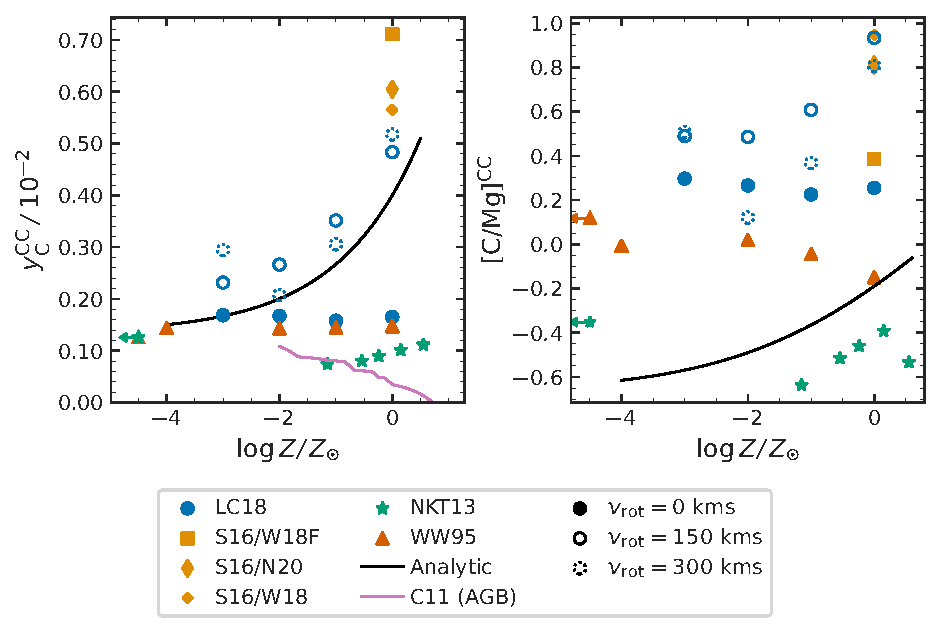
\includegraphics{cc_yields.pdf}
    \caption[]{
    \dbnote{might be interesting to plot every CCSNe yield used in this paper in light grey to show strength of our constraint}
        C yields from high-mass stars.
        \textbf{Left} The IMF-weighted \cc\ yield of C as a function of metallicity.
        \textbf{Right} The \cc\ [C/Mg] abundance ratio, defined in Eq.~\ref{eq:c_mg_cc}. The black line is the derived C yield from section~\ref{sec:mcmc_results}. Yields are shown for tables from 
    \citet[red triangles]{WW95}, \citet[orange square and diamond]{sukhbold+16}, 
    \citet[green stars]{NKT13}, and \citet[blue circles]{LC18}. \citet{sukhbold+16} report yields for different black hole landscapes, while \citet{LC18} provide yields at different rotational velocities.
    In the left panel, the pink line denotes $\Ycagb$ from \fruity{} for comparison. All models include wind yields. 
}
    \label{fig:y_cc}
\end{figure*}


\subsection{Supernova Type Ia}
The population averaged SN Ia yield, $y_{X}^{\rm ia}$, is given by,
\begin{equation}
    y_{X}^{\rm Ia} = m_{X}^{\rm Ia} \frac{N_{\rm Ia}}{M_\star}
\end{equation}
where $m_{X}^{\rm Ia}$ is the average mass of $X$ produced in a single SN Ia event, and $N_{\rm Ia} / M_\star$ is the number of such events per unit mass of star formation. \dbstrike{The latter can be expressed as an integral over the SN Ia delay-time-distribution (DTD), which describes the rate at which stellar populations produce X through SN Ia in \VICE.} Following \citet{james+23}, we use a $t^{-1.1}$  delay time distribution (DTD) with a minimum delay-time of 150 Myr, based on comparisons of the SN Ia rate as a function of redshift and the cosmic SFR (e.g. \citealt{maoz+12}). 

Supernovae type Ia produce negligible C. For our adopted yield scale, the highest magnitude CCSNe yield of the models from iwamoto99 is $1.1\times10^{-4}$, corresponding to about 4\% of our total C production, however most models predict a \ia\ C yield of less than $0.4 \times 10^{-4}$. We do check that including this contribution negligibly impacts our results, so we neglect SNIa C production for simplicity.

Novae are important contributes of \C[13], but produce far less \C[12] \dbadd{CITE}.



\section{The Multi-zone Model}\label{sec:vice}

Our models extends the \citet[hereafter \JJ]{james+21} Milky Way model, run with the publicly available Versatile Integrator for Chemical Evolution (\VICE).%
    \footnote{\VICE~is available at \url{https://github.com/giganano/VICE}}
This model is described extensively in \JJ~and concisely summarized  in \citet{james+23}. Here, we provide a brief overview of the relevant model components.

Classical, \textit{one-zone} models of chemical evolution assume instantaneous mixing of metals in the star-forming ISM\ \citep[e.g.][]{matteucci21}. This simple framework is a poor approximation of the Milky Way.  The Galaxy evolves \textit{inside-out} -- where star formation is higher towards the center and in the early universe \citep{WF91, kauffmann96, bird+13}. Stars can also migrate several kpc over their lifetimes, mixing different chemical environments across the galaxy \citep{bird+12,sellwood+binney02}. To account for different environments and stellar migration, multi-zone models stitch together multiple one-zone models and mix stellar populations between zones. \dbnote{does this belong in intro or here?. Thinking here now because feels more like methodology justification, but not sure still.}


The Galaxy is divided into 200 rings, each representing a single, 100\,pc zone. Each ring (or zone) has a separate stellar population and gas supply. We initially assume an inside-out SFH from \JJ, where the star formation surface density $\dot{\Sigma}_\star$ is given by 
\begin{equation}\label{eq:inside_out}
    \dot{\Sigma}_\star \propto \left(1-e^{-t/\tau_{\rm rise}}\right) e^{-t/\tau_{\rm sfh}}.
\end{equation}
$\tau_\text{rise}=2$\,Gyr loosely describes when the star formation rate reaches a maximum, and $\tau_{\rm sfh}$ describes the decay timescale of star formation as a function of radius $R$. \JJ\ derive $\tau_{\rm sfh}(R)$ through analysis of four integral field spectroscopy surveys in \cite{sanches20}. At each $R$, the SFH is normalized to match the stellar surface density gradient \citep{BHG16} assuming a total stellar mass of $5.17\times10^{10}\,\Mo$ \citep{LM15}. Star formation ends beyond a radius $R=15.5\,$kpc, but stellar populations are allowed to migrate as far as $R=20\,$kpc.  
The gas inflow is calculated to maintain the SFH for each radius and time, using an extension of the Kennicutt-Schmidt law \citep{kennicutt98} motivated by the combined observations of \citet{bigiel+10} and \citet{leroy+13}, 
\begin{equation}
\dot{\Sigma}_{\star} \propto 
\begin{cases}
    {\Sigma}_{\rm gas} & 2\times 10^7 \Mo\,{\rm kpc}^{-2} \leq \Sigma_{\rm gas} \\ 
    {(\Sigma}_{\rm gas})^{3.6} & 5\times 10^6 \Mo\,{\rm kpc}^{-2}\leq \Sigma_{\rm gas} < 2\times10^7 \Mo\,{\rm kpc}^{-2}\\ 
    {(\Sigma}_{\rm gas})^{1.7} & \Sigma_{\rm gas} < 5\times10^6 \Mo\,{\rm kpc}^{-2}.
\end{cases}
\end{equation} 
The scaling of this relationship varies with time due to the redshift dependence of $\tau_\star$ in molecular gas observed by \citet{tacconi18}.


We use the radial migration prescription described in appendix C of \citet{dubay+24}.\footnote{Not shown here, we also explored variations of temporal, spatial resolution, migration strength, and the mass lifetimre relation. We found these do not affect median trends significantly.}
We do not account for radial gas flows.
Not shown here, we also explore migration based on random walks and the \texttt{h277} hydrodynamical
simulation results\footnote{(with simulation parameters as in \citealt{bird+21}; see also \citealt{christensen12, zolotov12, loebman12, BZ14} \dbnote{is this okay as footnote?} }, which leaves our qualitative conclusions unchanged. 
The full impact of the details of a galaxy's dynamical history on its chemical evolution is still unknown.

As the strength of outflows controls the resulting $\alpha$-element abundances, we extend \JJ and create a metallicity gradient by defining
\begin{equation}\label{eq:mass_loading}
\eta(R) = \frac{y_{\alpha}^{\rm cc}}{Z_{\alpha}(R)} -1 + r + \tau_{\star} / \tau_{\rm sfh} 
\end{equation}
where 
\begin{equation}
    \log Z_{\alpha}(R) = \log Z_{\alpha,\ \odot} + 
    0.29 + 
    \begin{cases}
        -0.015(R-5) & R < 5 \\
        -0.09(R-5) & R \geq 5
    \end{cases}
\end{equation}
is adapted from \citet{hayden+14}.  We approximate $r=0.4$, and $\tau_\star/\tau_{\rm sfh} = 0.0$ .
This choice of $\eta(R)$ results in a [$\alpha$/H] gradient consistent with Milky Way observations \citep[e.g.][]{hayden+14, weinberg+19, frinchaboy+13}.
If we change our assumed $y_{\rm Mg}$, the values of $\eta$ will change similarly to maintain the correct chemical trends.

To create representative stellar samples to compare with APOGEE, 
we draw \nsubgiants\ stars from the simulated stellar populations. First, we draw a random zone (weighted by number of subgiants in zone) and then draw a random particle in the zone weighted by SSP mass.
Galactocentric radii are taken from astroNN \citep{leung+bovy19, leung+bovy19b}, however Gaia parallaxes yield a similar distribution. Alternative distributions of stars (including uniform distributions in 7-9kpc) minimally affect median trends.

\subsection{Monte-Carlo Markov Chain Yield Inference} \label{sec:mcmc_methods}

In GCE, total elemental abundances are (to first order) linear with respect to combinations of yields \citep[e.g.][]{WAF17}.
\dbnote{might be useful to include a complete set of differential equations for our model somewhere to better illustrate this.}
Assume that the yields do not depend on the yields (e.g. metallicity dependence is negligable). 
Given a set of yields $\{y_X^i\}_i$ and resulting abundance evolution $\{Z_{X}^i(R, t) \}$, let $y_X'$, the yield of X, be a linear combination of $\{y_X^i\}$
\begin{equation}
    y_X' = \sum_i \alpha_i\, y_X^i \quad {\rm where\ } \alpha_i \in \mathbb{R}.
\end{equation}
Then the abundance evolution of element $X$ is
\begin{equation}\label{eq:lin_combo}
    Z_X'(R, t) = \sum_i \alpha_i Z_X^i(R, t).
\end{equation}
Therefore, we can efficiently explore combinations of yields without the need for full simulations. This allows for direct observational inference of the yield combinations which best agree with the data.
We use Monte Carole Markov Chain (MCMC) inference to generate the posterior distributions of yield coefficients. Note that many other GCE parameters are nonlinear with abundance and require full multi-zone simulations, such as star formation history, outflows, and migration prescriptions. 
Also note that metallicity-dependent yields also introduce a second-order effect (metallicity depends on yields which depend on metallicity).

Our first step is to run a multi-zone model tracking the abundances of each process we are interested in. 
We focus on the binned \textit{mean} abundances of the low-$\alpha$ sequence in \caah, and the $-0.15 \leq {\rm [M/H]} \leq -0.05$ metallicity slice in \caafe\ (with 20 bin edges between -0.4 and 0.3 in [Mg/H] and 12 bin edges between 0.025 and 0.25 in [Mg/Fe]).
We separate the C yield  into four different components.
\begin{enumerate}
    \item $\alpha$: Prefactor for an AGB yield table
    \item $\zetao$: Constant CCSN yield  ($y_0 = \zeta_0$)
    \item $\zetai$: Linear CCSN yield ($y_1 = \zeta_1 \log Z/\Zo$) \footnotemark{}
    \item $\zetaii$: Quadratic CCSN yield ($y_2 = \zeta_2 (\log Z/\Zo)^2$)
\end{enumerate}
The total C abundances for a linear of these yields is given from Eq.~\ref{eq:lin_combo}.
Since we are taking means of each bin, there is a statistical uncertainty associated with the mean in a given bin, $\sigma_{i, \rm model}$. The total variance of the combined yield model is 
\begin{equation}
    \sigma^2_{\rm model} = \sum_{i} \alpha_i^2 \sigma^2_{i, \rm model}
\end{equation}
Similarly, we represent the mean and variance of the observations in each bin $b$ with $\bar Z_{b, \rm obs}$ and $\sigma^2_{b, \rm obs}$.  
\begin{equation} \label{eq:mcmc_likelihood}
    \log {\cal L} \propto \chi^2 = \sum_b \frac{(\bar Z_{b,\rm\ model} - \bar Z_{b,\rm\ obs})^2} {\sigma_{b, \rm tot}^2}
\end{equation}
where the total variance in a bin is 
\begin{equation}
    \sigma_{b, \rm tot} = \sigma_{\rm int}^2 + \sigma_{b, \rm obs}^2 + \sigma^2_{b, \rm model}
\end{equation}
where we model $\sigma_{\rm int}^2$ as a free parameter in the model.
\footnotetext{In detail, $y_1$ and $y_2$ are held constant past $\log Z/\Zo < -2$ and the $y_1$ component is modelled with a positive constant offset later subtracted to avoid negative abundances.}

We adopt the following priors
\begin{subequations}
\begin{align}
    \alpha &\sim N(1, 1) \\
    \zeta^{(0)} &\sim N(2, 1) \\
    \zeta^{(1)} &\sim N(0, 1) \\
    \zeta^{(2)} &\sim N(0, 4) \\
    \ln \sigma _{\rm int}&\sim N(-3, 1) \\
\end{align}
\end{subequations}
We run the MCMC using Turing.jl with a No-U-turn sampler (acceptance rate of 0.65), combining 16 independent chains with 3,000 steps each for a total of 48,000 samples.

To ensure this method is relatively robust, we will perform similar MCMC simulations varying the bin size and method, the MCMC sampler (Halmotonian, ensemble stretch moves from python-emcee, Metropolis-Hastings, Metropolis-Hastings random walk), the likelihood (including median U test, t-test, and KL-divergence based instead of mean + variance), and explore 2D bin likelihoods. In each case, the derived parameters are within their uncertainties (excluding the KS-divergence model).  We check that removing the likelihood in \caafe{} causes $\alpha$ to become unconstrained, as $\alpha$ is degenerate with the CCSN yields in \caah.


\section{Results}\label{sec:results}

\subsection{Evolution of Carbon Abundances}

\begin{figure*}
\centering
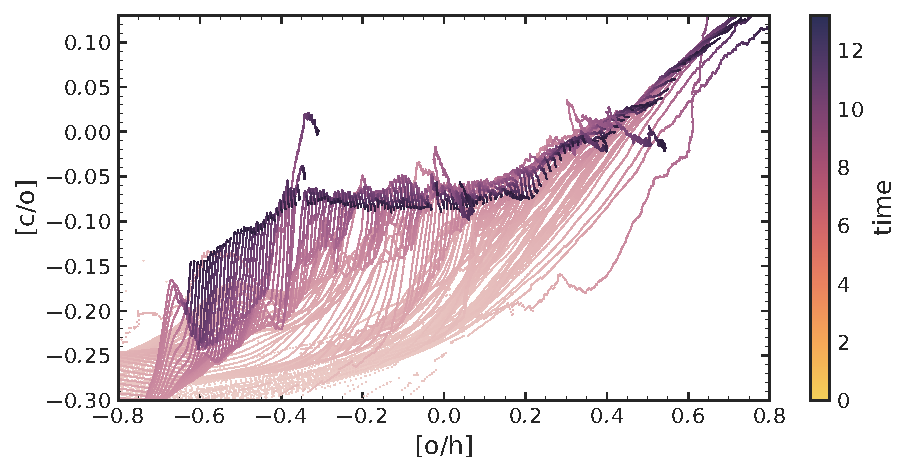
\includegraphics{figures/all_the_tracks.pdf}
\caption[]{
    Time evolution of gas-phase C abundances in our fiducial model for [C/Mg] versus [Mg/H] (left) and [Mg/Fe] (right).
    Each line represents a zone at a different galactic radius and is colour-coded by time. While \caah\ settles into the final trend $\sim{8}$\,Gyr ago, \caafe\ continues to evolve for much longer.
    \dbnote{radii between 2kpc and 15.5 kpc ?}
    \dbnote{add equilibrium lines (green?)}
}
\label{fig:c_evo}
\end{figure*}

% \begin{figure*}
%     \centering
%     \includegraphics{figures/subgiants_equilibrium_reproduced.pdf}
%     \caption{
%     Similar to Fig.~\ref{fig:subgiants} except for the stars of our fiducial model. 
%     The solid, black lines show the equilibrium abundance track. The black scatter points with errorbars are the median bins for the low-$\alpha$ sequence (left) and the \caafe\ trend (right). The green solid line on the right shows the singlezone evolution of \caafe\ with properties matching our solar-annulus. The median trend of low-$\alpha$ stars is an excellent approximation for the equilibrium abundance of C. 
%     \dbnote{The more I look at this figure, maybe we just add green lines to Fig. 5 and skip this one}
%     \dbnote{we add synthetic scatter found by fitting the metallicity-dependent reported errors with a linear fit in APOGEE and adding gaussian noise.}
%     \dbnote{is there too much going on here?}
%     \dbnote{would it make sense to maybe place this fig close to Fig.~1 since they are very similar so it is easier to compare? Not sure how to make continuity work then..}
%     \label{fig:equilibrium_validity}
%     }
% \end{figure*}



Fig.~\ref{fig:c_evo} shows evolutionary tracks for every zone of the fiducial model.
\caah\ trend quickly reaches our equilibrium state in \about{5}\,Gyr. \caafe\ tracks continue to evolve due to the long tail in the DTD of \ia. 


The evolution of abundances in our fiducial model is as follows:
\begin{enumerate}
    \item[(1)] {\it CCSN phase.} Star formation begins. Initially, \cc\ dominate enrichment. [C/Mg] evolves with yields set by $\Ycc/\Yoc$, resulting in increasing values with [Mg/H].  [Mg/H] quickly approaches its equilibrium value, but Fe remains low in comparison (in agreement with \citealt{WAF17}).
    \item[(2)]  {\it AGB/SN Ia phase.} A few hundred million years later, delayed sources enrich the ISM. \agb\ stars release C, raising [C/Mg], and \ia\ expel Fe, lowering Mg/Fe. 
    \item[(3)] {\it Approach to equilibrium.} Several billion years later, [C/Mg] plateaus as C also approaches equilibrium. [Mg/H] reaches equilibrium. [Fe/H] continues to increase due to ongoing \ia\ from old stellar populations. 
    \item {\it Present day.} The abundances of C, Mg, and Fe reach their equilibrium values. 

\end{enumerate}
This evolution is predominantly driven by our chosen elemental yields, their
metallicity dependence, and their DTDs.
As we will demonstrate in section~\ref{sec:agb_results} below, the final slope of \caah\ depends on both the contributions and metallicity dependences of CCSN and AGB C yields. Although AGB models predict declining C production with metallicity, the greater contribution and positive metallicity dependence of CCSN C outweigh declining AGB production.



 Fig.~\ref{fig:c_evo} {\color{red} will} show the  equilibrium tracks in \caah\, and \caafe. Based on the \citepos{WAF17} analytic models of chemical equilibrium for constant star formation, the equilibrium abundance ratio between two elements depends only on the relative yields. For C/Mg, 
\begin{equation}\label{eq:equilibrium_yields}
    {\rm [C/Mg]_{eq}} \equiv \log \left(\frac{\Ycc + \Ycagb }{y_{\rm Mg}}\right) - \log \left(\frac{Z_{\rm C,\,\odot}}{Z_{\rm Mg,\,\odot}}\right)
\end{equation}
As such, the equilibrium abundance represents the steady-state expectation for C abundances.  
However, in the \caafe\ plane, the equilibrium track is constant in [Mg/Fe] and only appears as a vertical line representing the range of equilibrium [C/Mg] values. The trends in \caafe\ are instead representative of the temporal evolution of [C/Mg].  \caafe\ is well approximated by either a single-stellar-population or a single zone model because of the shallow metallicity gradient of the Milky Way. \dbnote{is this right?}


\subsection{Yield Variations}\label{sec:results_highmass}
\label{sec:agb_results}

\begin{figure*}
    \includegraphics{sims_zeta_f.pdf}
    
    \caption[]{
        Stellar abundance trend predictions of our models . Coloured lines represent the median [C/Mg] in bins of [Mg/H] (left) or [Mg/Fe] (right) for each \agb\ table. Black points and grey dashes represent the median and 16th-84th percentiles of [C/Mg] in each bin in the \citet{jack}~sample. 
        The left panel only shows low-$\alpha$ stars. In the right panels, we show the trends only for stars where $-0.15\leq {\rm [Mg/H]}\leq -0.05$.
        Stars are binned into 20 (left) or 12 (right) equal number bins. 
        \textbf{Top}: Models with different metallicity dependences for  \cc\ C yields. \textbf{Bottom}: Models with different AGB C fractions $\fagb$ (only changing $\aagb$ and $\zetao$).
    }
    \label{fig:zeta_f}
\end{figure*}




The top of Fig.~\ref{fig:zeta_f} shows models with varying strengths of the $\Ycc$ metallicity dependence, $\zcc$. With higher $\zcc$, the model predicts a steeper \caah\ trend, owing to the direct relationship between the C/Mg equilibrium abundances and yield ratios. 
However, \caafe~is minimally affected by changes to $\zcc$ for stars at a given [Mg/H].
CCSN occurs on much shorter timescales than AGB and SN Ia enrichment, so CC carbon reaches equilibrium before delayed C and Fe production modifies trends. 
\footnote{The only effects on \caafe, when considering the narrow metallicity slice, are because of either the systematic change in equilibrium abundances, the imperfect evolution of the galaxy, or that the ISM abundances are set by stars which were born at poorer metallicities. }


The bottom of Fig.~\ref{fig:zeta_f} shows three models with different C \agb\  fractions, defined as 
\begin{equation}\label{eq:f_agb}
    \fagb \equiv \frac{\Ycagb(\Zo)}{\Yct(\Zo)}.
\end{equation}
Modifications of $\fagb$ affect both \caafe\ and \caah. At fixed metallicity, the \caafe\ trend is principally sensitive to how much C and Fe comes from delayed sources. Increasing the \agb\ fraction therefore steepens the \caafe\ trend as expected. Though each yield model predicts the trend to flatten at ${\rm [Mg/Fe]} \lesssim 0.1 $, the median is still within the width of the observed distribution and the overall agreement is good. Additionally, increasing \agb\ contribution to C leads to a declining net slope for the total C yield owing to the negative slope of \agb\ C production with metallicity.

\subsection{Yield Inference Results} \label{sec:mcmc_results}


\begin{figure}
\centering
\includegraphics{figures/mcmc_corner.pdf}
\caption[]{
A corner plot of the posterior samples from the MCMC simulation for the fiducial + \fruity\ model fit to the binned mean trends.
$\alpha$ represents the scale factor for the AGB yields, and $\zetao$, $\zetai$ and $\zetaii$ represent the constant, linear, and quadratic components of the CCSN yield.
See section~\ref{sec:mcmc_methods} for a description of the methods.
}

\label{fig:mcmc}
\end{figure}


\begin{figure*}
    \centering
    \includegraphics[]{figures/mcmc_fagb.pdf}
    \includegraphics[]{figures/mcmc_y_tot.pdf}
    
    \caption[]{
    \textbf{Left:} Posterior distribution of $\fagb$ from MCMC samples for each model we show. Regardless of assumptions, the best values of $\fagb$ range from about 0.1 to 0.35 and in all cases is less than 0.5.
    \textbf{Right:} The final total C yield (CCSN + AGB) for the median parameters from MCMC fits for each model. Additionally, we show individual samples from the \fruity{} \ MCMC model as faint blue lines.
    \dbnote{mark alpha=1.}
    }
    
    \label{fig:mcmc_ytot}
\end{figure*}



Fig.~\ref{fig:mcmc} shows the distribution and correlation of each parameter in the fiducial MCMC model. Each parameter is relatively well-constrained. The most prominent correlation, between $\zetao$ and $\alpha$ represents the constraint on the equilibrium abundance of C near solar. The other main correlation, between $\zetai$ and $\zetaii$, arises from the shape of the \caah\ trend. If the quadratic component decreases, then the \caah\  slope (past [Mg/H] $\lesssim 0.1$) increases, so the linear component must decrease in order to maintain agreement with the data.

Table~\ref{tab:mcmc_results} contains the resulting posterior distributions for each parameter for a variety of both AGB models and GCE assumptions. 
For the fiducial model, the best fit yields are 
\begin{equation}
    \frac{\Ycc}{y_{\rm Mg}} = (2.01\pm  0.08) + (2.20 \pm 0.15) x + (2.73 \pm 0.31) x^2
\end{equation}
where $x = \log Z/\Zo$.
Fig.~\ref{fig:mcmc_ytot} shows the AGB fraction at solar metallicity and the total C yield with metallicity for each MCMC run. 
In essentially each case, the majority of samples have a AGB fraction between 0.15 and 0.4. 


\begin{table*}


    \caption{
    Best-fit parameters (medians and 16-84th percentile errors) from MCMC analysis for various models discussed.
    The columns are:  modelname \textit{model}, best fit reduced $\chi^2$, best fit log posterior probability $\log p$, AGB scaling $\aagb$, 
    \dbnote{Not sure if we should use analytic, nugrid, shifted fruity or normal fruity yields as fiducial for this section, e.g. for eta, lateburst, twoinfall, etc...}}
    \label{tab:mcmc_results}
{ 
\renewcommand{\baselinestretch}{1.2}
    \begin{tabular}{l l l l l l l l l l l} 
    \hline
    model            & $\chi2$  & $\log p$ & $\aagb$ & $\zetao$ & $\zetai$ & $\zetaii$ & $\sigma_{\rm int}$ & $\fagb$ & $\Yct$ & $\zeta_{\rm 1, tot}$\\
\hline
fruity           &      6.9 &    20.06 & $1.96^{+0.21}_{-0.21}$  &  $2.01^{+0.08}_{-0.08}$  &  $2.20^{+0.15}_{-0.15}$  &  $2.73^{+0.31}_{-0.31}$  &  $0.08^{+0.02}_{-0.01}$  &  $0.27^{+0.03}_{-0.03}$  &  $2.75^{+0.02}_{-0.02}$  &  $1.52^{+0.13}_{-0.13}$\\ 
fruity m0.7      &      6.3 &    28.60 & $1.10^{+0.10}_{-0.10}$  &  $2.33^{+0.04}_{-0.04}$  &  $1.71^{+0.11}_{-0.11}$  &  $2.89^{+0.27}_{-0.27}$  &  $0.06^{+0.01}_{-0.01}$  &  $0.17^{+0.01}_{-0.01}$  &  $2.80^{+0.01}_{-0.02}$  &  $1.37^{+0.10}_{-0.10}$\\ 
aton             &     10.5 &    10.66 & $1.56^{+0.24}_{-0.24}$  &  $2.50^{+0.04}_{-0.04}$  &  $3.37^{+0.32}_{-0.32}$  &  $2.50^{+0.40}_{-0.39}$  &  $0.11^{+0.02}_{-0.02}$  &  $0.08^{+0.01}_{-0.01}$  &  $2.72^{+0.02}_{-0.02}$  &  $1.81^{+0.17}_{-0.17}$\\ 
monash           &     10.8 &     6.86 & $2.06^{+0.37}_{-0.39}$  &  $1.92^{+0.16}_{-0.15}$  &  $3.68^{+0.42}_{-0.45}$  &  $3.52^{+0.47}_{-0.47}$  &  $0.13^{+0.03}_{-0.02}$  &  $0.23^{+0.05}_{-0.05}$  &  $2.49^{+0.05}_{-0.05}$  &  $1.41^{+0.20}_{-0.19}$\\ 
nugrid           &      6.1 &    23.68 & $1.00^{+0.10}_{-0.10}$  &  $1.75^{+0.10}_{-0.10}$  &  $1.58^{+0.12}_{-0.12}$  &  $3.19^{+0.31}_{-0.30}$  &  $0.07^{+0.02}_{-0.01}$  &  $0.32^{+0.03}_{-0.03}$  &  $2.58^{+0.02}_{-0.02}$  &  $1.12^{+0.12}_{-0.13}$\\ 
analytic         &      5.1 &    29.80 & $0.43^{+0.04}_{-0.04}$  &  $2.33^{+0.04}_{-0.04}$  &  $1.57^{+0.10}_{-0.10}$  &  $2.69^{+0.27}_{-0.26}$  &  $0.06^{+0.01}_{-0.01}$  &  $0.15^{+0.01}_{-0.01}$  &  $2.75^{+0.01}_{-0.01}$  &  $1.15^{+0.10}_{-0.11}$\\ 
eta2             &      6.6 &    24.28 & $0.47^{+0.05}_{-0.04}$  &  $2.24^{+0.05}_{-0.05}$  &  $1.45^{+0.09}_{-0.10}$  &  $2.95^{+0.32}_{-0.32}$  &  $0.07^{+0.02}_{-0.01}$  &  $0.17^{+0.02}_{-0.02}$  &  $2.71^{+0.02}_{-0.01}$  &  $0.98^{+0.09}_{-0.09}$\\ 
lateburst        &      8.0 &    21.72 & $0.56^{+0.05}_{-0.05}$  &  $2.25^{+0.05}_{-0.05}$  &  $1.75^{+0.18}_{-0.18}$  &  $2.55^{+0.37}_{-0.36}$  &  $0.08^{+0.02}_{-0.01}$  &  $0.20^{+0.02}_{-0.02}$  &  $2.81^{+0.02}_{-0.02}$  &  $1.19^{+0.18}_{-0.18}$\\ 
twoinfall        &      6.3 &    17.12 & $0.54^{+0.06}_{-0.06}$  &  $2.31^{+0.07}_{-0.07}$  &  $1.72^{+0.19}_{-0.20}$  &  $1.69^{+0.30}_{-0.30}$  &  $0.09^{+0.02}_{-0.02}$  &  $0.19^{+0.02}_{-0.02}$  &  $2.85^{+0.02}_{-0.03}$  &  $1.18^{+0.20}_{-0.20}$\\ 
fruitylin       &    &    & $1.95$  &  $2.10^{+0.02}_{-0.02}$  &  $1.55^{+0.08}_{-0.08}$  &     &  $0.09^{+0.02}_{-0.01}$  &  $0.26^{+0.00}_{-0.00}$  &  $2.84^{+0.02}_{-0.02}$  &  $0.87^{+0.08}_{-0.08}$\\ 
analyticlin     &    &    & $0.43$  &  $2.41^{+0.02}_{-0.02}$  &  $0.89^{+0.09}_{-0.09}$  &     &  $0.10^{+0.02}_{-0.01}$  &  $0.15^{+0.00}_{-0.00}$  &  $2.84^{+0.02}_{-0.02}$  &  $0.46^{+0.09}_{-0.09}$\\ 
\hline
total & &   &  -  &  $2.26^{+0.11}_{-0.37}$  &  $1.74^{+1.53}_{-0.24}$  &  $2.79^{+0.49}_{-0.58}$  &  $0.08^{+0.03}_{-0.02}$  &  $0.19^{+0.09}_{-0.04}$  &  $2.74^{+0.07}_{-0.16}$  &  $1.26^{+0.32}_{-0.24}$\\
\hline
    \end{tabular}

}
    
\end{table*}


\subsection{Unknowns and Degeneracies} \label{sec:sfh} \label{sec:outflows}
\label{sec:degeneracies}

\begin{figure*}
    \includegraphics{figures/zeta_f_mass_sfh.pdf}
    
    \caption[]{
        Similar to Fig.~\ref{fig:zeta_f}, except for \caafe\ for a variety of models.
        {\bf Left} models where both the \agb\ fraction and the CCSNe slope are varied simultaneously.
        {\bf Middle} models where the \agb\ yields are shifted by some factor in mass.
        {\bf Right} alternate star formations and a model where yields and outflows are $\sim$ doubled.
    \dbnote{update caption here}
    }
    \label{fig:sims_degens}
\end{figure*}

\begin{figure*}
    \includegraphics[]{figures/mcmc_caahfe_predicted.pdf}

    \caption[]{
        Similar to Fig.~\ref{fig:zeta_f} except showing the mean tracks for different best-fit AGB yield tables with best-fit CCSNe parameters. Variations in the \caafe\ plane are due to the different total AGB C yield and variations in the mass-dependence of each yield table.
    \dbnote{use actual best fit median trends here instead of inferred yields? Update labels, remove one of analytic / fruity m0.7}.
    }
    \label{fig:agb_predictions}
\end{figure*}

Assumptions about the AGB yields, the star formation history, and outflows negligibly impact \caah\ due to chemical equilibrium. However, these degeneracies can inform and affect the interpretation of \caafe. 

Because both the increase in \cc\ slope $\zcc$ and AGB fraction $\fagb$ have similar impacts to \caah, we can change both parameters simultaneously to retain agreement in \caah. We show example models in the left panel of Fig.~\ref{fig:sims_degens} in \caafe, (as models cannot be readily distinguished in \caah). The principle effect of increasing $\fagb$ and adjusting $\zcc$ correspondingly is to increase the amplitude of the trend in \caafe. Models with little to no AGB C production will produce stars with [C/Mg] independent of [Mg/Fe] in a metallicity slice. As the AGB fraction increases to an extreme $f^{\rm AGB}=0.5$, the trend becomes steeper than the fiducial but remains a rescaling of the same shape. 


A second factor affecting \caafe\ is the assumed delay time distribution of \agb\ carbon production.
The middle panel of Fig.~\ref{fig:sims_degens} shows models where the AGB yields have been shifted by a factor in mass. When the AGB C production is weighted towards more massive AGB stars, then the delay time distribution becomes more rapid, causing equilibrium to be reached sooner (at higher [Mg/Fe]). The \caafe\ trend therefore is less sensitive to the C production by stars with masses $M \gtrsim 5 \Mo$ \dbnote{calculate timescales here}. On the other hand, shifting the C production towards low mass stars extends the DTD towards longer times. In Fig.~\ref{fig:sims_degens}, models shifted towards lower masses increase the amplitude of the \caafe\ trend, particularly steepening the high [Mg/Fe] slope. For the most extreme case, where the masses are shifted by a factor of 0.5; the AGB production is more delayed than SNeIa, causing an increasing slope of \caafe\ towards low [Mg/Fe]. An intermediate mass shifts (0.7) is approximant linear in \caafe, qualitatively matching the observed trend. 

Fig.~\ref{fig:agb_predictions} shows the resulting median trends in \caah\ and \caafe\ for the median parameters for each AGB model. Regardless of the AGB model, there is a reasonable choice of \cc\ yields which can closely match the \caah\ trend. All AGB models predict similar \caafe\ trends. However, each (unshifted) yield table underpredicts the slope of \caafe\ at low [Mg/Fe]. As discussed above, the relative flattening in \caafe\ results from a AGB DTD that is more prompt than SNe Ia.
Also, note that the median parameters (from Table~\ref{tab:mcmc_results}) suggest an amplification of AGB yields of between 1.5 and 2 for all models except \nugrid. Without this amplification, the overal trend in \caafe\ would be much flatter than is observed. 
We suggest that most AGB yield models require an increase in the amplitude of C production and a weighting of C production more towards low mass stars in order to better match observations in this GCE framework.


We consider two alternative SFHs. 
Motivated by the findings of \citet[see discussion in \JJ]{mor+19,isern19}, the \textit{lateburst} model
adds a Gaussian burst to the fiducial inside-out model, 
\begin{equation}\label{eq:lateburst}
    \dot{\Sigma}_\text{lateburst} \propto \dot{\Sigma}_\text{inside-out} \left(1 + A\,e^{-(t-\tau_{\rm burst})^2/2\sigma^2_{\rm burst}} \right)
\end{equation}
where $A=1.5$ represents the amplitude of the birth, $\tau_\text{burst}=10.8$\,Gyr is the time where the burst is strongest, and $\sigma_\text{burst}=1$\,Gyr is the width of the burst.

We also consider a two-infall like model as presented in \dbadd{dubay + 24}, which is defined as.
\begin{equation}\label{twoinfall}
\dot{\Sigma}_{\rm in} \propto e^{-t/\tau_1} + A \theta(t - t_{2}) e^{-t/\tau_2}
\end{equation}
where $\tau_1=\#\,$Gyr, $\tau_2=4\,$Gyr, $A=\Sigma_{\rm thin} / \Sigma_{\rm thick}$ \dbadd{explanation}, $t_2=4$, and the star formation also abruptly transitions from $\nu=2$/Gyr to $\nu=1$/Gyr at $t=t_1$?

The right panel of Fig.~\ref{fig:sims_degens} compares the fiducial, lateburst, and two-infall models. The pertubations to \caafe\ are small. The largest change is to the distribution of [Mg/Fe], but the \caafe\ trends are identical for the lateburst or is slightly shifted and steeper for the two infall model. So, variations due to SFH considered here are most likely smaller than width of the observed distribution.
Building on \citet{james+23}, we conclude that the \caah\ and \caafe\ trends reflect nucleosynthetic yields more than the Galactic SFH. 
\dbnote{There has to be a good reason why \caafe\ is not affected or maybe only more extreme pertubations make a difference?}



While some Milky Way \gce{} models (including ours) incorporate significant mass-loading, others
neglect mass-loading and instead use lower yields \citep[e.g.][]{MCM13, MCM14, spitoni19, spitoni20, spitoni21}.
Both classes of models are able to reproduce many details of the disk abundance structure due to the strong degeneracy between the normalizations of elemental yields and mass-loading (see discussion in, e.g. \citealt{sandford+24} and Appendix B of \citealt{james+23}). 
Our parameterization of $\eta$ illustrates this (see Equation~\ref{eq:mass_loading}) -- choosing a lower value of $y_{\alpha}$ will similarly result in lower values of $\eta$ while maintaining the same metallicity gradient. 
We consider a model where we double all yields, in the right panel of Fig.~\ref{fig:sims_degens}. A uniform change in yields and outflows leaves our median trends relatively unchanged. 
\dbnote{This paragraph is slightly off, the actual value of eta around the sun is only 0.5 so reducing outflows more does not keep metallicity gradient. Do we need to change framing here?}


Additionally, Fe yields and the \ia\  delay-time-distribution have their own uncertainties. Increasing both $y_{\rm Fe}^{\rm Ia}$ and $\Ycagb$ correspondingly leaves \caafe\ mostly unchanged. Not shown here, if both processes increase by a similar proportion of the total yield, then our predictions in \caafe\ are unchanged. Therefore, we cannot know the DTD of C more accurately than that of Fe in this framework.

\dbnote{Other things to discuss possibly ? :
 Initial mass function (and possible metallicity dependence)? ISM stochasticy and inhomogeneities. Metallicity-Dependent Oxygen/Magnesium and Iron yields? Gas phase migration / ISM cooling?  mass-lifetime relation. Spectroscopic systematics.
 }


\subsection{Nitrogen}


\begin{figure}
\centering
\includegraphics{figures/nitrogen.pdf}

\caption[]{Similar to Fig.~\ref{fig:zeta_f} except for [C/N] against [Mg/H] for the fiducial model. Combining our results with the suggested yield from \JJ\ (rescaled to our adopted yields) explains both the thin-disk evolution of C and N. 
}
\label{fig:nitrogen}
\end{figure}

N production, also affected by the CNO cycle, is closely tied to C. As a test of our model, we use the \agb\ N yield suggested by \citet{james+23}. Fig.~\ref{fig:nitrogen} shows [C/N] versus [Mg/H] and for our fiducial model. We are able to closely match the [C/N]-[Mg/H] trend. 
\dbnote{sentence about [C/N]-[Mg/Fe]}



\section{Gas-Phase Abundances}\label{sec:gas}

\begin{figure*}
\centering
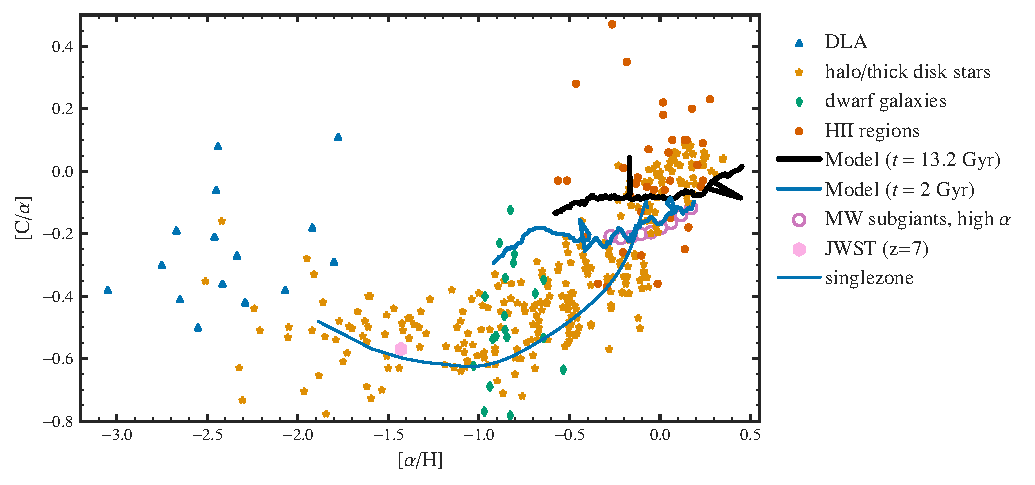
\includegraphics[]{figures/summary.pdf}
\caption[]{
\dbnote{will probably add each SZ model description to fig caption. Should citations be moved outside of caption for reader's sake?}
\dbnote{remove connecting lines on MW HII regions. Should I plot outliers at all?}.
Gas-phase C abundances. 
We plot the fiducial model's present-day ISM abundances as a thick blue line.
Black lines are single-zone models: a fiducial yields and MW-like model (solid black), and three corrected yield models representing the MW (dotted), GSE (dashed) and Wukong (dash-dots).
Points represent measurements in 
    MW HII regions \citep[orange circles][]{mendez-delgado+22}
    extragalactic RL HII regions \citep[green circles;][]{peimbert+05, skillman+20, toribio-san-cipriano+16, toribio-san-cipriano+17, esteban+14, esteban+09}
    extragalactic CEL HII regions \citep[green diamonds;][]{garnett+95, senchyna+17, izotov+thuan99, garnett+99, berg+16, berg+19, pena-guerrero+17}
    damped Lyman-alpha (DLA) systems \citep[rust triangles;][]{omera+01, cooke+14, welsh+22, ellison+10, welsh+20, cooke+18, riemer-sorensen+17, DZ+03, cooke+17, cooke+11, dutta+14, morrison+16, srianand+10, pettini+08, kislitsyn+24, cooke+15}, 
    Milky Way stars \citep[yellow stars;][]{amarsi+19},
    and high redshift galaxies \citep[pink squares, CEL lines;][]{steidel+16, stark+14, matthee+21, mainali+20, jones+23, amorin+17, iani+23, james+14, erb+10, bayliss+14, berg+18, christensen+12, arellano-cordova+2022}.


}

\label{fig:gas_phase}
\end{figure*}
% \begin{table}
% 	\centering
%     \caption[]{Single zone model parameters. \dbnote{change dwarf parameters to match Wukong from James' dwarf paper.  $\eta=47.99\pm 5$, $t_{\rm end} = 3.36\pm 0.5$, $\tau_\star=44.97\pm 7$, $\tau_{\rm sfh} = 3.08\pm 1$}}
% 	\label{tab:singlezone_params}
% 
% 	\begin{tabular}{l l l l l}
% 		\hline
%         Model & $\eta$ & $t_{\rm end}$ & $\tau_\star$ & $\tau_{\rm sfh}$ \\
% 		\hline
%         1 & 0.5 & 13.2 & 2.5 & 14\\
%         2 & 1 & 10 & 2 & 10\\
%         3 & 9 & 3 & 5 & 3\\
% 	\end{tabular}
% \end{table}

As a final test of our model, we compare the predictions against C abundances
in the gas phase. Besides stellar observations, C has been observed in extragalactic HII regions, high redshift galaxies (HII regions), metal-poor stars, and Damped-Lynman-$\alpha$ systems (DLAs).\footnote{DLAs are gas clouds observed as absorption spectra in front of background quasars}
While we used Mg as our representative alpha element in our APOGEE sample, O
is more readily observed in the gas-phase, so we shift focus to C/O in this
section.
HII measurements of C are challenging since C lacks strong recombination lines (RL)
 and its collisional excited lines (CEL) fall in the far ultraviolet without nearby reference H lines \citep[][]{skillman+20}.
Furthermore, CEL and RL derived abundances are systematically discrepent by \about{0.5}\,dex \citep{GR07}.
Metals may also be trapped in dust grains or in unobserved ionization states, requiring additional modeling \citep{MM19}.
As a consequence, the uncertainties of HII abundances are substantial (see representative error bars on Fig.~\ref{fig:gas_phase}).
\dbnote{
There is a complication I have not done that CEL and RL abundances (especially for O) need to be put on the same scale with +0.2 dex corrections. Probably need to double check derivations of metallicities...
}. DLAs, on the other hand, are relatively precise because these regions are lower-ionization, have a well-defined region (column density) and often have high-quality spectra covering rest-frame UV and optical {\color{red} CITE/verify}.

Fig.~\ref{fig:gas_phase} compiles literature measurements of DLAs, HII regions (MW, extragalactic, dwarfs), high redshift galaxies, and MW halo/thick disk stars. Despite the inhomogeneities, uncertainties, and variety of systems, there is still a coherent global trend.
Near solar metallicities, most observations (from disky galaxies) have near-solar [C/O].
As metallicity decreases, [C/O] also decreases, reaching a minimum of \about{-0.6} around ${\rm [O/H] \sim -1}$. Finally, [C/O] appears to increase again at the lowest metallicities observed (${\rm [M/H] \lesssim -2}$).

Fig.~\ref{fig:gas_phase} also shows the present-day gas phase abundance of our fiducial model and several single-zone models. The gas phase predictions of our multizone model agree reasonably with MW (and similar metallicity extragalactic) HII regions. Stellar abundance remain, comparatively, a more stringent constraint. To better represent the evolution of low-metallicity and dwarf galaxy environments, we create an illustrative suite of single-zone models. These models evolve only a single, homogenous gas supply. We assume a constant star formation efficiency $\dot M_\star = M_{\rm gas} / \tau_\star$. We also use an exponential infall history for dwarf galaxies of the form
\begin{equation}
    \dot\Sigma_{\rm in} \sim e^{-t/\tau_{\rm sfh}}.
\end{equation}
Yields are set to the best-fit analytic AGB model, but low metallicity evolution is predominantly driven by the choice of CCSNe C yields. We introduce an alternate CCSNe model to better agree with these low-$Z$ observations.
\begin{equation} 
    \Ycc / 10^{-3} = \begin{cases}
        0.8 & \log Z / \Zo < -1.81 \\
        2.41 + 0.89\, \log Z / \Zo & {\rm otherwise }
    \end{cases}
\end{equation}
where the low-metallicity limit was chosen to match the approximate minimum of observed [C/O] values.
The models shown in Fig.~\ref{fig:gas_phase} have the parameters: 
\begin{enumerate}
    \item Fiducial MW. Solid black line. $\eta=0.5$, $t_{\rm end} = 13.2$, $\tau_\star=2$, $\tau_{\rm sfh} = 14$, insideout SFH.
    \item Corrected MW-like. Dotted. Same parameters as  fiducial single-zone but with corrected yields.
    \item Corrected Gaia-Sausage Enceledus like. Dashed. $\eta=5.74$, $t_{\rm end}=10.73$, $\tau_\star = 26.60$, $\tau_{\rm sfh} = 2.18$, infall mode
    \item Corrected Wukong-like. Dash-doted. $\eta=28.8$, $t_{\rm end} = 3.36$, $\tau_\star=44.97$, $\tau_{\rm sfh} = 3.08$, infall mode
\end{enumerate}
\dbnote{check timescales to metallicity = -1 (could sagb affect the trends here?). Also try different yield sets for these just to see if any agree naturally... }

When comparing the MW-like single-zone model to the fiducial final gas-phase abundances, notice that the slope of the singlezone track near solar metallicities is steeper. 
While the trend in the multi-zone models arises as a
superposition of end-points, the single-zone trend instead arises as an evolutionary sequence (see Fig.~\ref{fig:c_evo}). The increase in [C/O] abundances is a result of both delayed AGB contribution and the metallicity-dependent C CCSNe yields.
The halo and thick disk stars also support that the past [C/O] abundances were increasing with metallicity, in contrast to the near-constant [C/O] of the low-$\alpha$ sequence.
The initial [C/O] value of these single-zone mdoel is governed by the respective ratio of C to O yields. As a result, the fiducial yield set predicts too high of a minimum [C/O], motivating our corrected yields. With the corrected yield set, the single-zone models are able to reproduce the general trend of [C/O] with metallicity.
An alternative explanation is that more C comes from delayed sources than is predicted by our fiducial model. However, reaching the [C/O] minimum of -0.6 requires that \about{75\%} of C comes from AGB stars, which is not reconcilable with the stellar \caafe\ trend.  

SFH variations likely explain part of the observed scatter in Fig.~\ref{fig:gas_phase}. 
In our models, variations in the SFHs change when [C/O] begins to increase with metallicity and the final [C/O] value of the model. Similar to [O/Fe] trends with metallicity, the slower and burstier SFH of dwarf galaxies causes delayed sources to affect abundance ratios at a lower metallicity than for MW-like systems.

Our single-zone models do not capture the elevated [C/O] ratio at the lowest metallicities. This could be remedied by modifying our CCSNe yield, but low-metallicity C abundances are beyond our scope. Additionally, inhomogeneous mixing and individual contributions from supernovae become important in this regime, adding additional scatter and complexity to modelling.
\dbnote{Are CEMPs worth mentioning here? since they have enough literature although not necessarily relavent here. Carigi+Peimbert 2011, Molla+2015.}

Altogether, our yields (with some adjustments) are able to reproduce the global C trend from dwarf galaxies to solar metallicity MW-like galaxies. 




\section{Discussion \& Conclusions}\label{sec:conclusions}


Building on~\citet{james+23}, we quantify the impact of C yield assumptions on Milky Way GCE models. We use \citepos{jack} sample of APOGEE subgiants as our primary observational benchmark, as subgiant atmospheres most likely reflect their birth C abundances (see discussion in section~\ref{sec:data_selection}).
In our fiducial model, C initially increases following the slope of the \cc\ C dependence. Later, AGB contributions from C cause a sharp rise in \caah, which slows down due to declining AGB C production and the approach towards equilibrium. The chemical elemental reach a quasi-equilibrium within \about{5}\,Gyr. As a result, the current C/Mg versus metallicity gradient is a superposition of equilibrium states, mixed together from different Galactic positions.


The slope of the predicted \caah\ relation is principally sensitive to the collective metallicity dependence of \cc\ C yields.
While AGB yields are predicted to decline with metallicity, out models show that \cc\ dominate the trend and make an overall positive metallicity trend. 
As the strength of the \cc\ metallicity dependence increases, the slope of the \caah\ trend correspondingly increases. The small effects of \agb\ C yield on the \caah\ trend can be easily corrected by small adjustments of the \cc\ yield's metallicity dependence.
Our predicted slope of NUMBER is approximately consistent with the \citet{LC18} rotating stellar models, however no simulation contains sufficient mass resolution or accuracy to reproduce the observed trends accurately. 

Because massive star enrichment dominates the C mass budget in our models, the predictions are relatively insensitive to the choice of AGB star yield model.
Of the \agb\ tables tested here, \fruity, \monash, and \nugrid\ all predict similar abundance trends in [C/Mg] with [Mg/H] and [Fe/Mg]. The strong destruction of C by massive stars at \about{} solar metallicity   in \aton\ are instead in tension with the data (See Figs.~\ref{fig:agb_predictions})  and~\ref{fig:agb-ssp})
As both the \fruity\ and \nugrid\ models predict \about{} linear N yields as well, these combined models best explain combined C and N abundance trends (see Appendix!?).

As in~\citet{james+23}, we have constrained yield ratios as opposed to absolute yields. For example, scaling yields and outflows by a corresponding factor leaves abundance ratio trends unchanged (Fig.~\ref{fig:sims_degens}).  Effects such as black hole formation could create systematic shifts on predicted chemical yields.
Variations in the SFH instead only induce minor systematic shifts


When combined with~\citeauthor{james+23}'s~\citeyearpar{james+23} empirically calibrated N yields, we find that our fiducial model accurately describes the [C/N]-[Mg/H] relation in our sample. The [C/N]-[Mg/Fe] relation, on the other hand, is shallower than the data, indicating that the DTD of C production may be sharper than our AGB yield tables would suggest (or the N DTD more extended, or both).

Finally, we compare our models againsts a compilation of literature gas-phase and halo-star abundances (see Fig.~\ref{fig:gas_phase}). Our fiducial model fails to explain the lowest values of [C/O] at metallicities of -1 to -2. We briefly consider a modified variation of the CCSNe yield of C which drops to explain these values, which maintains trends consistant with APOGEE. 


Our results demonstrate the power of empirically calibrated stellar yields. In our GCE models, trends in abundance ratios with metallicity are largely determined by trends in yield ratios with metallicity. As a result, the metallicity dependence of the total, population-averaged C yield is tightly constrained by the [C/Mg]-[Mg/H] relation, but the metallicity dependencies of the individual contributions from CCSNe and AGB stars are less precisely determined. Due to the sensitivity of elemental yields to poorly understood processes, such as mass-loss rates and convection, our results provide a useful benchmark for stellar evolution models~\citep[see the discussion in e.g.][]{gil-pons+2022}. With abundance measurements for several million stars provided by upcoming spectroscopic surveys, particularly SDSS-V's Milky Way Mapper program~\citep{sdssv}, constraints on both stellar nucleosynthesis and the assembly history of our Galaxy will become increasingly more powerful.

More C observations across different galactic environments will continue to refine a complete understanding of C production, including the yields of the first stars,  evolution in the bulge, and so on. 



\section*{Acknowledgements}

Software that has contributed to this work included  
\VICE~\citep{JW20, james+21},
\textsc{matplotlib} \citep{matplotlib},
\textsc{scipy} \citep{scipy},
\textsc{IPython} \citep{ipy},
\textsc{pandas} \citep{pandas},
\textsc{numpy} \citep{numpy},
\textsc{astropy} \citep{astropy:2013, astropy:2018, astropy:2022},
and 
\textsc{seaborn} \citep{seaborn}
.
Additionally, we thank \citet{OhioSupercomputerCenter1987} for the use of its facilities for the simulations. 

\apogee\ is part of SDSS-IV \citep{sloan_telescope, apogee_instrumentation, sdss_iv_overview, sdss17, apogee17, aspcap}.

Funding for the Sloan Digital Sky 
Survey IV has been provided by the 
Alfred P. Sloan Foundation, the U.S. 
Department of Energy Office of 
Science, and the Participating 
Institutions. 

SDSS-IV acknowledges support and 
resources from the Center for High 
Performance Computing  at the 
University of Utah. The SDSS 
website is www.sdss4.org.

SDSS-IV is managed by the 
Astrophysical Research Consortium 
for the Participating Institutions 
of the SDSS Collaboration including 
the Brazilian Participation Group, 
the Carnegie Institution for Science, 
Carnegie Mellon University, Center for 
Astrophysics | Harvard \& 
Smithsonian, the Chilean Participation 
Group, the French Participation Group, 
Instituto de Astrof\'isica de 
Canarias, The Johns Hopkins 
University, Kavli Institute for the 
Physics and Mathematics of the 
Universe (IPMU) / University of 
Tokyo, the Korean Participation Group, 
Lawrence Berkeley National Laboratory, 
Leibniz Institut f\"ur Astrophysik 
Potsdam (AIP),  Max-Planck-Institut 
f\"ur Astronomie (MPIA Heidelberg), 
Max-Planck-Institut f\"ur 
Astrophysik (MPA Garching), 
Max-Planck-Institut f\"ur 
Extraterrestrische Physik (MPE), 
National Astronomical Observatories of 
China, New Mexico State University, 
New York University, University of 
Notre Dame, Observat\'ario 
Nacional / MCTI, The Ohio State 
University, Pennsylvania State 
University, Shanghai 
Astronomical Observatory, United 
Kingdom Participation Group, 
Universidad Nacional Aut\'onoma 
de M\'exico, University of Arizona, 
University of Colorado Boulder, 
University of Oxford, University of 
Portsmouth, University of Utah, 
University of Virginia, University 
of Washington, University of 
Wisconsin, Vanderbilt University, 
and Yale University.

\dbnote{do I need acknowledgments for appendix spectro-surveys?}

%%%%%%%%%%%%%%%%%%%%%%%%%%%%%%%%%%%%%%%%%%%%%%%%%%
\section*{Data Availability}

\dbadd{data and codes used in this paper are all publicly available. (do i need links here?). }


%%%%%%%%%%%%%%%%%%%% REFERENCES %%%%%%%%%%%%%%%%%%
\bibliographystyle{mnras}
\bibliography{main}


%%%%%%%%%%%%%%%%% APPENDICES %%%%%%%%%%%%%%%%%%%%%

\appendix


\section{Model parameters and details}

\begin{table}
	\centering
    \caption[]{Description of the models presented in this paper.}
	\label{tab:model_parameters}

	\begin{tabular}{l l l l l l l l l l}
		\hline
            name & $\alpha_{\rm C}^{\rm AGB}$ & $Y_{\rm C}^{\rm AGB}$ & $\zeta_0$ & $\zeta_1$ & $\zeta_2$ \\ 
            \hline
            fiducial & 1.95 & fruity & 2.01 & 2.19 & 2.72 \\
            Monash & 2.06 & monash & 1.92 & 3.68 & 3.52 \\
            ATON & 1.56 & aton & 2.50 & 3.37 & 2.50 \\
            NuGRID & 1.00 & nugrid & 1.75 & 1.58 & 3.19 \\
            steep & 1.95 & fruity & 2.01 & 3.0 & 2.72 \\
            shallow & 1.95 & fruity & 2.01 & 1.0 & 2.72 \\
            f=0.1 & 0.721 & fruity & 2.47 & 2.19 & 2.72  \\
            f=0.4 & 2.88 & fruity & 1.64 & 2.19 & 2.72 \\
            f=0.1, zeta & 0.721 & fruity & 2.47 & 1.75 & 2.72  \\
            f=0.4, zeta & 2.88 & fruity & 1.64 & 2.51 & 2.72 \\
            m0.5 & 2.23 & fruity(m/0.5)  & 2.27 & 1.60 & 2.23 \\
            m0.7 & 1.73 & fruity(m/0.7) & 2.08 & 1.83 & 3.31 \\
            m1.5 & 2.12 & fruity(m/1.5) & 2.02 & 1.98 & 2.27 \\
		\hline
	\end{tabular}
\end{table}



For our added scatter, we use the polynomial fits to the reported internal APOGEE error with metallicity. In detail, these polynomials should also very with logg, teff, however as all of our stars are subgiants, these effects should be smaller. We also use $x={\rm [Fe/H]}$ for brevety.
\begin{subequations}
\begin{align}
    \delta {\rm [Mg/H]} &= 0.0652 x^2 + 0.00522 x + 0.0338 \\
    \delta {\rm [Mg/Fe]} &= 0.00793 x^2 - 0.00802 x + 0.0138 \\
    \delta {\rm [C/Mg]} &= -0.0378x + 0.03506 
\end{align}
\end{subequations}

Low-$\alpha$ stars are defined to have 
\begin{equation}\label{eq:high_alpha}
\begin{cases}
\text{[Mg/Fe]} <0.16-0.13\,\text{[Fe/H]}, & \text{[Fe/H]}<0\\
\text{[Mg/Fe]} <0.16, & \text{[Fe/H]}>0. \\
\end{cases}
\end{equation}



\section{NuGrid Yield Tables} \label{sec:nugrid_yields}
In this section, we present updated calculations of the \citep{battino+19, battino+21} yield tables and describe their incorperation into VICE.

\citep{battino+19, battino+21} update the \citep{ritter+18} yield models with new reaction rates and increased mixing. These changes allow for better production of {\it s}--process isotopes in their AGB stars, and are recommended for the masses they update. However, between these models, the only updates are for masses M=2,3 at metallicities Z=0.01, 0.02, 0.001, 0.002. 

Because the yield tables included in \citep{battino+19, battino+21} are inconsistent with the \citet{ritter+18} definitions of yields, we recalculate these yields from the publically available data on \url{https://astrohub.uvic.ca}. 

The total ejected mass of $X$ from an AGB star is given by 
\begin{equation}
    M_{X, \rm ej} = \int Z_{X, \rm surf}(t) \dot{m}(t)\ dt 
\end{equation}
where $Z_{X, \rm surf}$ is the surface abundance of $X$, $\dot m$ is the mass loss rate, and the integral is taken over the entire evolution. 
One complication is that MESA stops before the end of the AGB phase due to instabilities during the transition to the planetary nebulae. 
As a result, the practical calculation is 
\begin{subequations}
    \begin{align}
        M_{X, \rm ej} &= Z_{\rm X, surf, end} (m_{\rm end} - m_{\rm rem}) \\ 
                      &+ \sum_i \frac{1}{2} (Z_X(t_i) - Z_X(t_{i+1}))\ (m(t_i) - m(t_{i+1}))
    \end{align}
\end{subequations}
where $m_{\rm end}$ and $Z_{X, \rm surf, end}$ are the final mass and surface abundance of $X$ at the end of MESA evolution, $m_{\rm rem}$ is the mass remaining in the star at the end of MESA evolution, and the sum is taken over all timesteps in the MESA output. We use the final H-free mass as the reminant mass. 

We use the \citet{ritter+18} tables from $M_{X, \rm ej}$, which we can reproduce from the same methods as above. Finally, the $p_{X}$ yields are calculated from $M_{\rm X, ej}$ with Eq.~\ref{eq:stellar_yield_def}. 

\bsp	% typesetting comment
\label{lastpage}
\end{document}




